\documentclass[journal]{IEEEtran}
\usepackage{amsmath,amsfonts}
\usepackage{amssymb}
\usepackage{algorithmic}
\usepackage{algorithm}
\usepackage{array}
\usepackage[caption=false,font=normalsize,labelfont=rm,textfont=rm]{subfig}
\usepackage{iftex}
\ifXeTeX
  \usepackage{fontspec}
  \setmainfont{Times New Roman}
\fi
\usepackage{textcomp}
\usepackage{stfloats}
\usepackage{url}
\usepackage{verbatim}
\usepackage{graphicx}
\usepackage{booktabs}
\usepackage{cite}
\usepackage{placeins}
\usepackage{balance}
\ifXeTeX
  \usepackage{xeCJK}
  \setCJKmainfont{SimSun}
\fi
\usepackage{xcolor}
\definecolor{revisionred}{RGB}{190,0,0}
\definecolor{revisionblue}{RGB}{0,82,170}
\DeclareRobustCommand{\oldtext}[1]{{\color{revisionred}#1}}
\DeclareRobustCommand{\newtext}[1]{{\color{revisionblue}#1}}
\DeclareRobustCommand{\why}[1]{{\color{revisionblue}{\footnotesize (#1)}}}
\DeclareRobustCommand{\rw}[3]{\oldtext{#1} \newtext{#2}\why{#3}}
\hyphenation{op-tical net-works semi-conduc-tor IEEE-Xplore}
% updated with editorial comments 8/9/2021

% Float-page tuning: avoid small double-column figures occupying a nearly empty page.
\makeatletter
\setcounter{topnumber}{2}
\setcounter{dbltopnumber}{2}
\renewcommand{\topfraction}{0.9}
\renewcommand{\dbltopfraction}{0.9}
\renewcommand{\textfraction}{0.05}
\renewcommand{\floatpagefraction}{0.85}
\renewcommand{\dblfloatpagefraction}{0.85}
\setlength{\@fptop}{0pt}
\setlength{\@fpbot}{0pt plus 1fil}
\setlength{\@dblfptop}{0pt}
\setlength{\@dblfpbot}{0pt plus 1fil}
\makeatother

\begin{document}

\title{\rw{A Sample Article Using IEEEtran.cls\\ for IEEE Journals and Transactions}{A Plug-and-Play Stage-Wise Online Adaptation Framework for Load Forecasting Under Distribution Shift}{原题名是 IEEE 模板标题；修改为与稿件主题一致的工作题名，未加入未经证实的 SOTA 词汇。}}

\author{\oldtext{IEEE Publication Technology,~\IEEEmembership{Staff,~IEEE,}}\\
\newtext{Author names, affiliations, and IEEE memberships to be inserted after author confirmation}\why{原作者信息为模板占位；不能编造真实作者与单位。}
\thanks{\oldtext{This paper was produced by the IEEE Publication Technology Group. They are in Piscataway, NJ.} \newtext{Funding, data-source, and contribution acknowledgments should be inserted after verification.}\why{删除模板说明，保留需作者确认的信息槽位。}}
\thanks{\oldtext{Manuscript received April 19, 2021; revised August 16, 2021.} \newtext{Manuscript history will be supplied by the journal workflow.}\why{模板日期不可用于投稿。}}}

% The paper headers
\markboth{\newtext{Journal header pending final metadata}}%
{\newtext{Author et al.: Stage-Wise Online Adaptation for Load Forecasting}}

\IEEEpubid{\rw{0000--0000/00\$00.00~\copyright~2021 IEEE}{Publisher copyright line to be assigned after acceptance}{模板版权号不能作为投稿信息。}}
% Remember, if you use this you must call \IEEEpubidadjcol in the second
% column for its text to clear the IEEEpubid mark.

\maketitle

\begin{abstract}
\rw{This paper studies online multivariate regional load forecasting under delayed feedback and distribution shift.}{This paper studies multivariate regional load forecasting under distribution shift with a batch-delayed online adaptation protocol.}{把 delayed-feedback 改成与当前实现更一致的 batch-delayed protocol，避免严格逐时间戳反馈承诺。} We develop a plug-and-play forecasting framework that combines invariant representation learning, factor-based expert modeling, and a three-stage online controller. The framework separates stable predictive structure from variant fluctuations, performs relevance-guided sparse updates only when experts become unstable, and applies transient drift compensation at inference time. \rw{Extensive experiments on multiple load forecasting datasets and multiple transformer-based backbones show that the proposed framework consistently improves over frozen deployment and representative online baselines under shifted online streams.}{Experiments on the tested datasets and transformer-family backbones show improved performance over frozen deployment in the shifted-stream protocol and competitive behavior relative to the implemented online-adaptation baselines, with dataset-dependent rankings.}{删除 consistently 和 representative online baselines 的过度表述；保留已由审计支持的范围。}
\end{abstract}

\begin{IEEEkeywords}
online load forecasting, multivariate time series, distribution shift, invariant learning, transformer backbone, \rw{delayed feedback}{batch-delayed online adaptation}{关键词与实现协议保持一致。}.
\end{IEEEkeywords}



\begin{center}
\fbox{\parbox{0.94\linewidth}{\newtext{\textbf{Revision-scope note.} This marked-up version fixes wording, format, grammar, terminology, caption clarity, and evidence-scope statements that can be corrected without inventing new experiments or citations. Experimental-result limitations that require reruns, multi-seed evidence, faithful external baselines, or code/protocol changes are not fabricated here; they are reflected only as scoped wording or author-action notes.}\why{按用户要求，本稿只修可通过文本与格式处理的问题，不伪造实验改进。}}}
\end{center}
\noindent\rw{Journal of \LaTeX\ Class Files,~Vol.~14, No.~8, August~2021 / Shell et al.: A Sample Article Using IEEEtran.cls for IEEE Journals}{Journal header pending final metadata / Author et al.: Stage-Wise Online Adaptation for Load Forecasting}{原页眉为模板内容；实际作者和期刊元数据需作者确认后填写。}

\section{Introduction}
Regional load forecasting in real deployment environments is inherently nonstationary. Seasonal transitions, weather fluctuations, and changing demand patterns cause the online test stream to deviate from the distribution seen during offline training. In such settings, a strong offline forecaster alone is often insufficient, while \rw{naive online fine-tuning can be unstable under delayed labels and concept drift.}{unconstrained online fine-tuning can be unstable when labels are delayed and the deployment stream drifts.}{语法和措辞更正式，避免口语化 naive。} This motivates an online forecasting framework that can preserve stable mechanisms, localize unstable components, and adapt conservatively when the distribution shifts.

The method developed in this paper follows that principle. We first isolate invariant predictive structure through environment-aware representation learning, then model dynamic load-generation mechanisms through a factorized multi-expert forecasting backbone, and finally perform structured online adaptation through Stage~I, Stage~II, and Stage~III. \rw{Stage~I recalibrates the factor mixture under delayed labels, Stage~II performs relevance-guided sparse expert updates when instability is detected, and Stage~III applies transient correction based on the discrepancy between variant and invariant representations.}{Stage~I recalibrates the factor mixture when delayed labels become available, Stage~II performs relevance-guided sparse expert updates under the implemented acceptance gates, and Stage~III applies transient correction based on the discrepancy between variant and invariant representations.}{限定 Stage II 触发条件，避免把实现风险写成严格在线保证。}

Unlike methods tied to a single predictor, the proposed design is formulated as a plug-and-play framework. The same online controller can be combined with multiple transformer-based backbones, which allows the experiments to evaluate both forecasting strength and backbone generality. \rw{The following sections present the problem formulation, the method, and the empirical validation.}{The following sections present the formulation, model components, online protocol, and evidence-limited empirical evaluation.}{承认当前证据范围，降低“validation”过强语气。}

\section{Preliminaries}
\subsection{Notation}
Let $\{\mathbf{x}_t\}_{t=1}^{T}$ denote a multivariate time series, where $\mathbf{x}_t \in \mathbb{R}^{N}$ and $N$ is the number of observed variables. We formulate time-series forecasting via a sliding-window scheme: for each reference time $t$, an input lookback window of length $L$ is used to predict an output horizon window of length $H$. Specifically, we define the input window $\mathbf{X}_t \triangleq [\mathbf{x}_{t-L+1},\ldots,\mathbf{x}_t] \in \mathbb{R}^{L \times N}$ and the output window $\mathbf{Y}_t \triangleq [y_{t+1},\ldots,y_{t+H}] \in \mathbb{R}^{H}$, where $y_t$ denotes the target variable. The formulation extends directly to multivariate targets by letting $\mathbf{Y}_t \in \mathbb{R}^{H \times d_{\mathrm{out}}}$.

A forecasting model $f_{\theta}: \mathbb{R}^{L \times N} \rightarrow \mathbb{R}^{H}$ parameterized by $\theta$ maps past observations to future targets, and $\widehat{\mathbf{Y}}_t = f_{\theta}(\mathbf{X}_t)$. Given a pointwise loss function $\ell(\widehat{\mathbf{Y}}_t,\mathbf{Y}_t)$, standard training minimizes the empirical risk over the training set \rw{$\mathcal{D}_{\mathrm{tr}}=\{(\mathbf{X}_t,\mathbf{Y}_t)\}_{t=1}^{N}$}{$\mathcal{D}_{\mathrm{tr}}=\{(\mathbf{X}_j,\mathbf{Y}_j)\}_{j=1}^{M_{\mathrm{tr}}}$}{避免与变量数 $N$ 冲突，用 $M_{\mathrm{tr}}$ 表示训练窗口样本数。}, formulated as:  \rw{$\min_{\theta}\frac{1}{N}\sum_{t=1}^{N}\ell\big(f_{\theta}(\mathbf{X}_t),\mathbf{Y}_t\big)$}{$\min_{\theta}\frac{1}{M_{\mathrm{tr}}}\sum_{j=1}^{M_{\mathrm{tr}}}\ell\big(f_{\theta}(\mathbf{X}_j),\mathbf{Y}_j\big)$}{同步修正经验风险中的样本数记号。}.

\subsection{Online Learning in OOD Settings}
Let $P_{\mathrm{tr}}(X,Y)$ and $P_{\mathrm{te}}(X,Y)$ denote the joint distributions of input windows $X$ and targets $Y$ for training and test. OOD forecasting has $P_{\mathrm{te}}(X,Y)\neq P_{\mathrm{tr}}(X,Y)$ and can be characterized by the following shifts.

\textbf{Covariate shift.} $P_{\mathrm{te}}(X)\neq P_{\mathrm{tr}}(X)$; the input marginal changes, e.g., meteorological covariates differ across years or net-load profiles shift after large-scale renewable integration.

\textbf{Label shift.} $P_{\mathrm{te}}(Y)\neq P_{\mathrm{tr}}(Y)$; the target marginal changes, e.g., electrification increases mean load or industrial expansion alters peak frequency, causing bias under historical target density.

\textbf{Conditional shift.} $P_{\mathrm{te}}(Y|X)\neq P_{\mathrm{tr}}(Y|X)$; the mapping from history to future changes due to altered influence mechanisms among variables, e.g., demand response changes load sensitivity to temperature.

\textbf{Latent shift induced by unobserved variables.} Let $Z$ denote unobserved drivers affecting both $X$ and $Y$. Changes in $P_{\mathrm{te}}(Z)\neq P_{\mathrm{tr}}(Z)$ can induce joint shifts in observed variables. In load forecasting, such shifts may be triggered by extreme weather or public health emergencies, e.g., sudden demand changes beyond recorded covariates.

  \begin{figure}[!t]
  \centering
  \subfloat[\footnotesize \textbf{Conventional deep forecasting.} Conventional deep forecasters learn $P(Y|X)$ from historical data under $P_{\mathrm{tr}}(X,Y)$. When an unobserved driver $Z$ influences both $X$ and $Y$, a deployment shift in $P(Z)$ can induce changes in the effective conditional $P(Y|X)$, thereby breaking the training-stage relationship and degrading performance. ]
  {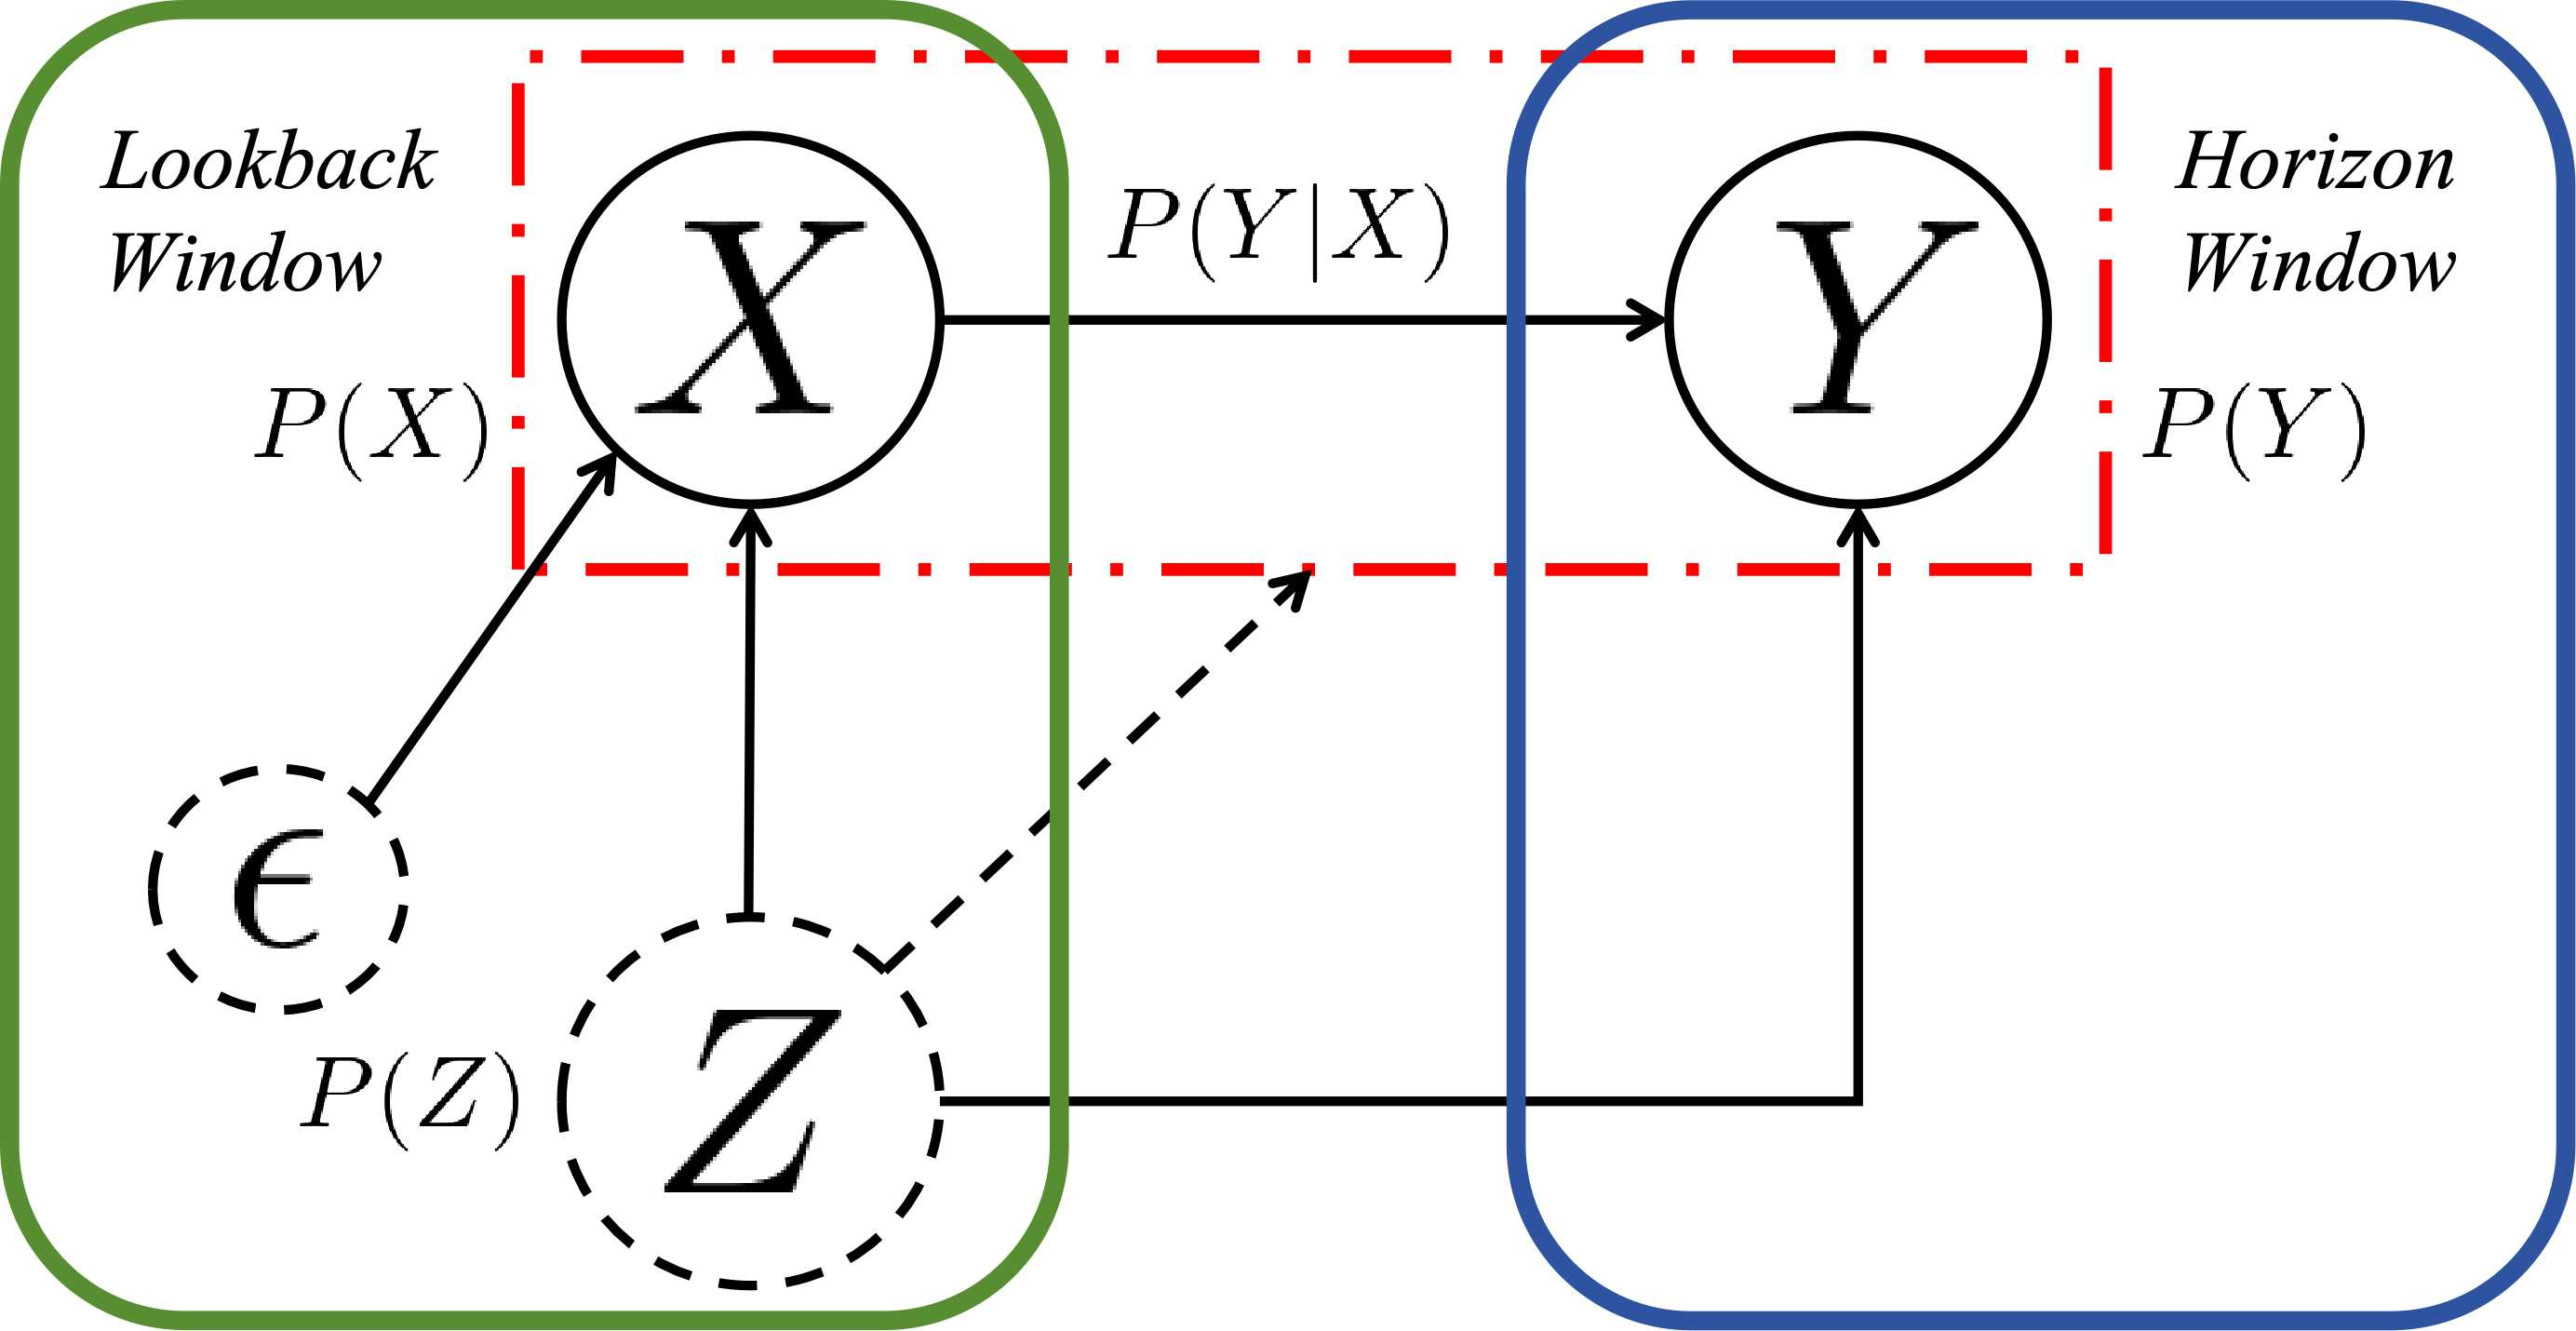
\includegraphics[width=0.8\linewidth]{fig2.jpg}\label{fig:dist_shift_b}}\\
  \vspace{0.5em}
  \subfloat[\footnotesize \textbf{Invariant learning module.}  ]
  {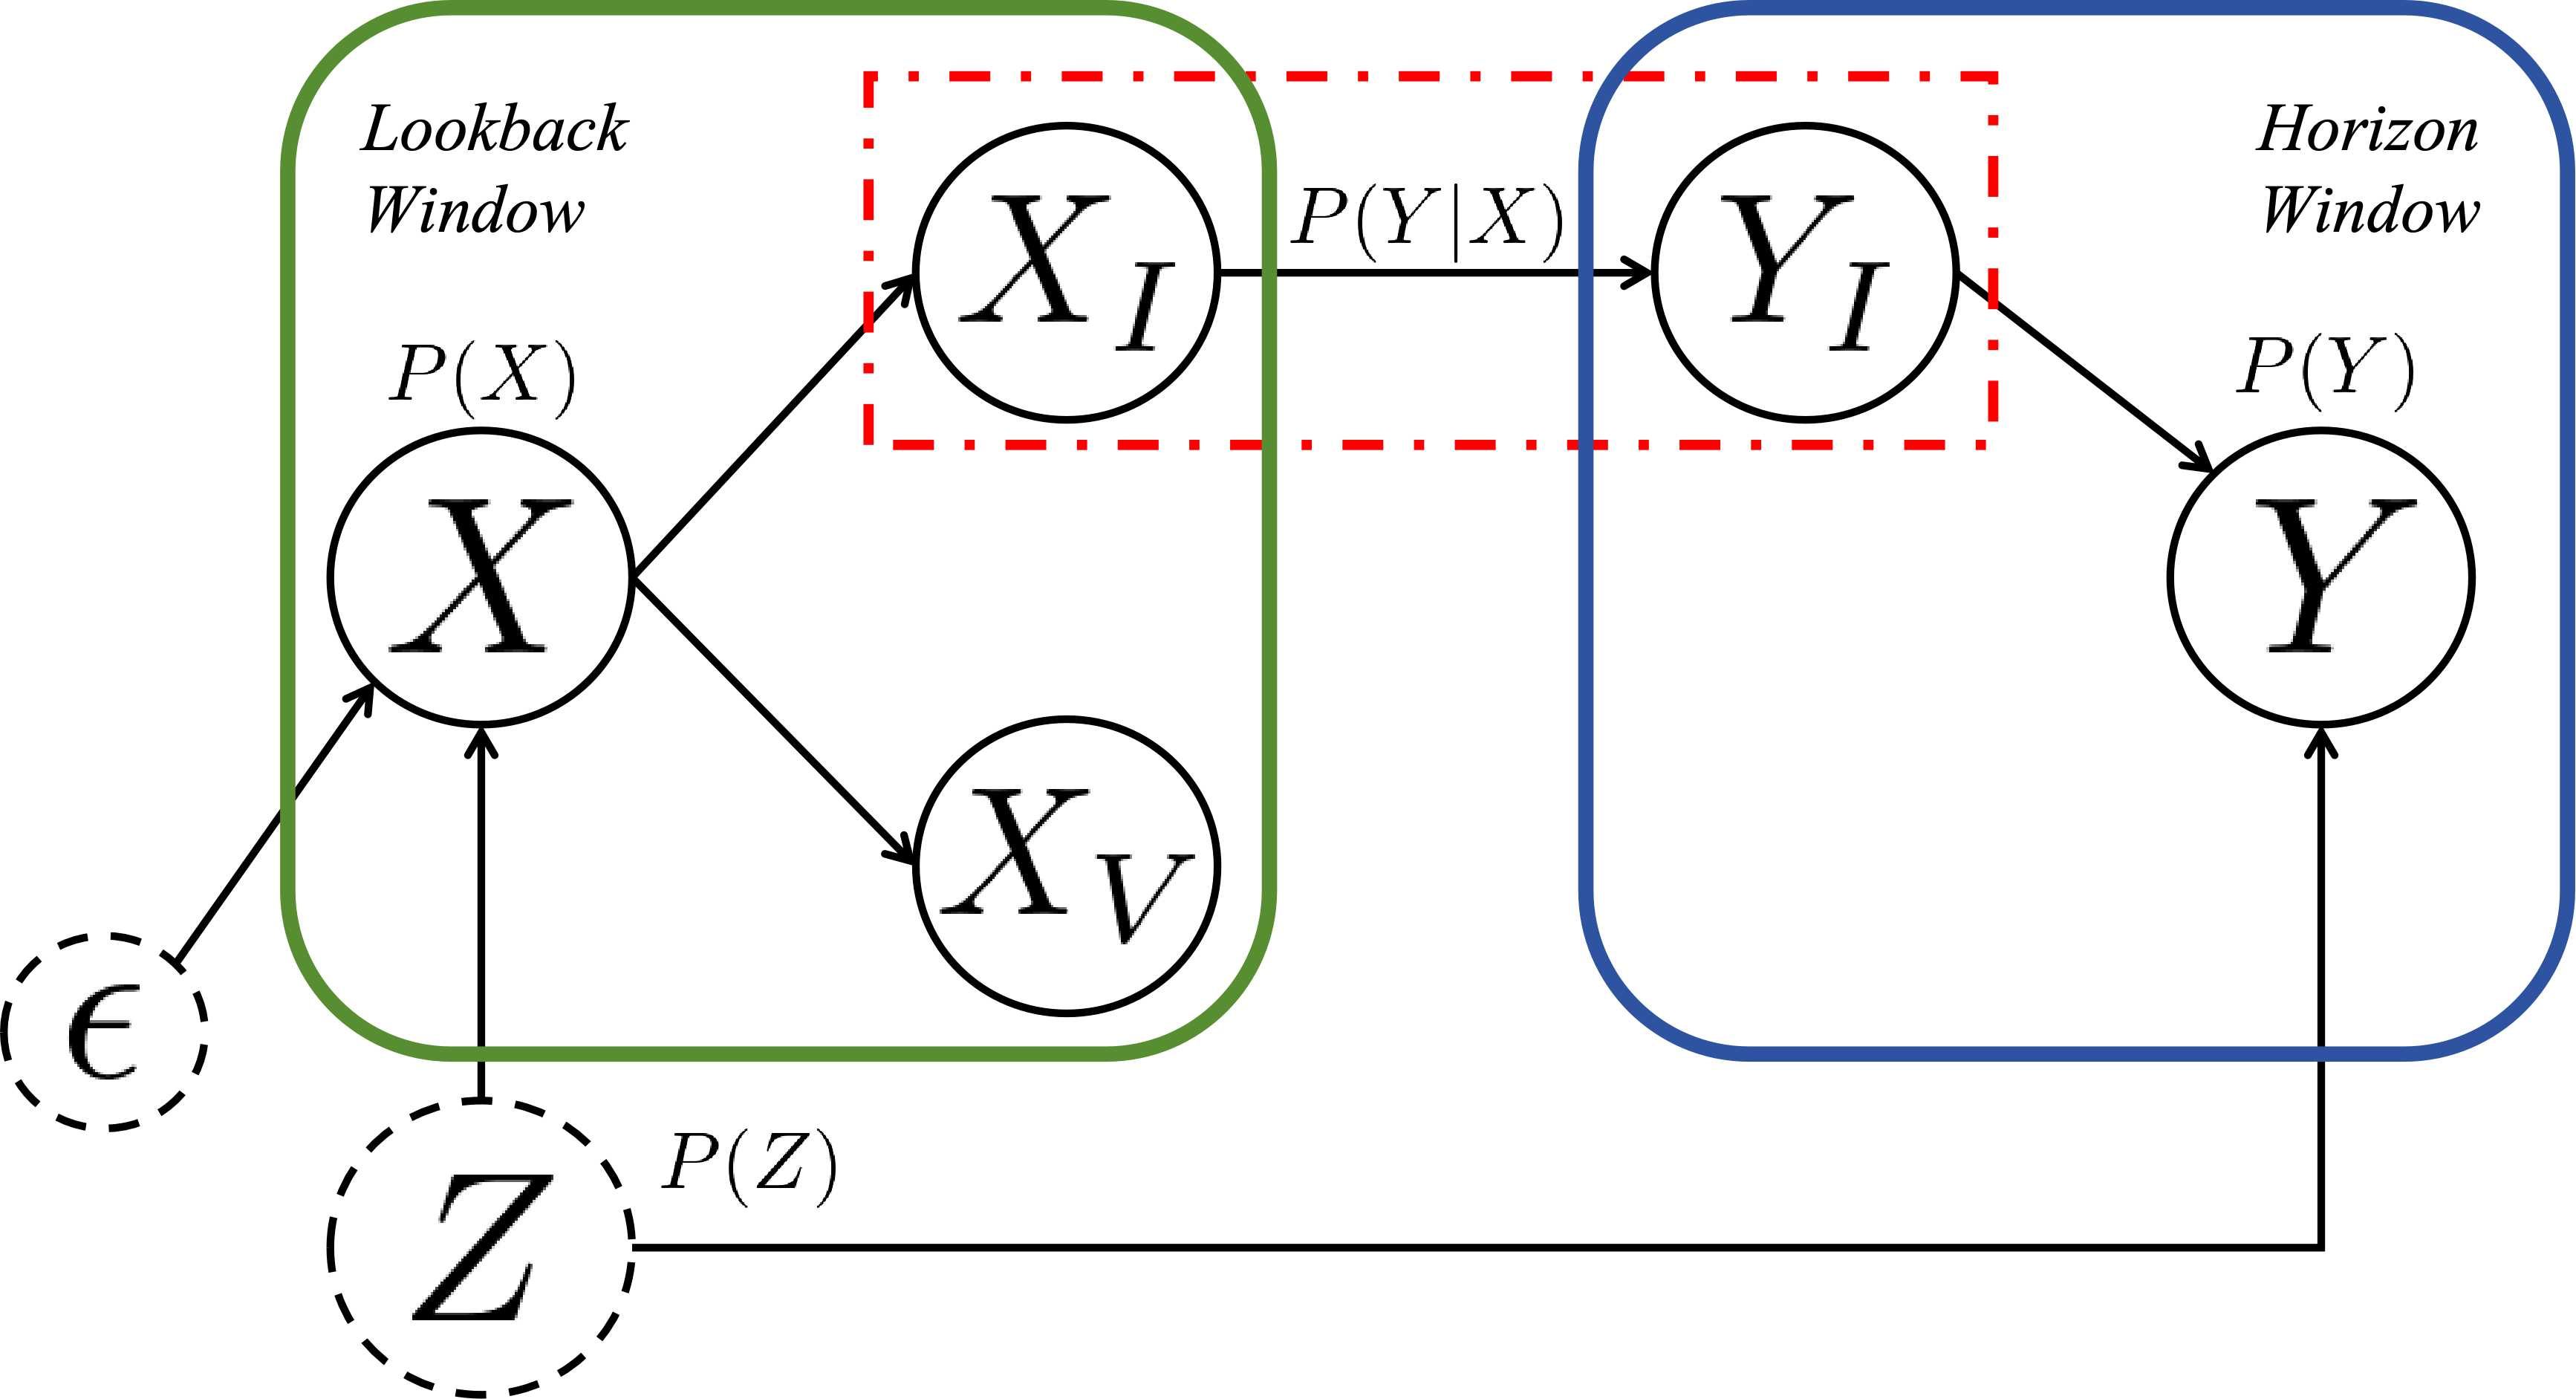
\includegraphics[width=0.8\linewidth]{fig1.jpg}\label{fig:dist_shift_a}}\\
  \caption{Examples of distribution shifts.}
  \label{fig:dist_shift}
  \end{figure}

In practice, multiple shift types can co-occur, complicating OOD generalization. This motivates online learning in OOD settings to mitigate distribution drift by continually transforming newly observed series into training samples and updating model parameters to minimize forecast errors on recent data. However, conventional online learning faces three structural constraints: (i) \rw{due to the feedback delay in Section~1, updates can only use labels arriving at least $L$ steps later}{because labels are available only after a feedback delay $D$, online updates can use only labels that have already arrived}{修复错误章节引用，并区分 lookback $L$ 与 feedback delay $D$。}; (ii) the online phase may encounter novel operating regimes outside the historical distribution. (iii) \rw{some distribution drift is caused by variant unobserved factors.}{some drift may be associated with unobserved or weakly observed drivers.}{避免在无因果识别证据时断言 drift 原因。} If updates are not applied selectively, the model can overfit and experience sustained performance degradation after the drift subsides. 

Therefore, a proactive online adaptation framework is needed to (i) enable rapid parameter adjustment under drift, and (ii) explicitly classify stable, long-term changes from fluctuations driven by variant unobserved factors, so that different online learning strategies can be applied accordingly.

\subsection{Structural Causal Model}

To provide a principled basis for such selective adaptation, \rw{Structural Causal Model (SCM) is introduced to represent latent drivers and causal mechanisms, providing a principled basis for reasoning. SCM consists of endogenous variables $V$, exogenous variables $U$, structural assignments $V_i \leftarrow f_i(\mathrm{Pa}(V_i), U_i)$ for each $V_i \in V$, and a joint distribution $P(U)$ over the exogenous variables. The directed graph induced by the parent sets $\mathrm{Pa}_i$ encodes direct causal effects among variables. The induced directed graph encodes direct causal effects.}{We use SCM terminology as conceptual motivation for separating stable and variant mechanisms. An SCM consists of endogenous variables $V$, exogenous variables $U$, structural assignments $V_i \leftarrow f_i(\mathrm{Pa}(V_i), U_i)$, and a joint distribution $P(U)$. In this manuscript, the SCM discussion motivates the model design; it should not be read as evidence that a causal graph is identified from the current experiments.}{删去重复句，并明确 SCM 是动机而非已验证的因果发现。}

\section{Methodology}
\subsection{Overview}
% To clarify the limitations of existing OOD forecasting frameworks and motivate our targeted improvements, the paper organizes this section around three research questions.

\oldtext{\textbf{RQ1:}}\newtext{ }\why{空白 RQ 占位删除；若保留，必须写成可由实验回答的研究问题。}

% For existing OOD frameworks, identifying $X_I$ and $Y_I$ from data is generally infeasible in practice due to unobserved drivers $Z$. How can we quantify the impact of $Z$ on $X$ and $Y$ and thereby obtain principled approximations of $X_I$ and $Y_I$?

\oldtext{\textbf{RQ2:}}\newtext{ }\why{空白 RQ 占位删除。}

% Learning a stable conditional relation $P(Y_I|X_I)$ is the primary objective for robust OOD forecasting. How should the stable relation $P(Y_I|X_I)$ be represented in a forecasting model, such that stability can be represented and enforced under distribution shifts?

\oldtext{\textbf{RQ3:}}\newtext{ }\why{空白 RQ 占位删除。}

% Urban load series are mixtures of heterogeneous components, each governed by its own stable interaction mechanism among variables. Consequently, the effective relation captured by training can be a superposition of multiple component specific conditionals $\{P_{f_i}(Y_I|X_I)\}$. How can we disentangle and learn these specific relations?

% This work targets robust Out-of-Distribution Short-term Urban Load Forecasting by developing an causality informed invariant learning framework, which learns a stable predictive relation $P(Y_I|X_I)$ between invariant features $X_I$ and the sufficiently predictable component $Y_I$ across different environments. Specifically, we apply the Fast Fourier Transform (FFT) to retain the top $K$ dominant frequency components, and define a unified Periodic Window (PW) using the Least Common Multiple (LCM) of their periods. The framework then partition each PW into Frequency Specific Sub-windows (FW) and use a multi branch architecture to extract frequency wise representations. Each branch is equipped with a Two-stage Attention layer to extract cross-time and cross-variable dependency. To promote the extraction of $X_I$, we compute cross-variable attention maps for FW in each frequency branch and maximize the similarity of maps at aligned time positions across adjacent PW. To approximate $Y_I$ and reduce the interference from unobserved drivers $Z$, we introduce Causal Directed Acyclic Graph (DAG) to quantify the causal contribution of the observed inputs $X$ and unobserved variables $Z$ to the target $Y$, and use the estimated strengths to reweight sample contributions in the training loss.

The methodology is organized as follows: invariant learning for stable components is defined first, followed by the factor-mechanism forecasting backbone, and finally the \rw{two-stage online adaptation}{three-stage online adaptation}{全文实际使用 Stage I/II/III，应统一为三阶段。}.

\subsection{\rw{The decomposition of ... using Invariant Learning}{Invariant Representation Learning for Stable and Variant Components}{替换占位标题，明确本节内容。}}
To separate long-term changes from variant fluctuations, an invariant learning module is introduced to extract features $\mathbf{X}_{\mathrm{I}}$ and a sufficiently predictable component $\mathbf{Y}_{\mathrm{suf}}$ whose conditional relation $P_e(\mathbf{Y}_{\mathrm{suf}}|\mathbf{X}_{\mathrm{I}})$ is invariant across environments (Fig.~1(b)). $\mathbf{X}_{\mathrm{I}}$ is the subset of inputs $\mathbf{X}$ that provides sufficient, environment-stable predictive information for $\mathbf{Y}_{\mathrm{suf}}$, and both are intended to exclude variant effects from unobserved factors. \rw{The following invariance assumption is adopted:}{We use the following working assumption to motivate the loss design:}{降低未经证明的“assumption adopted”语气。}

\begin{equation}
\mathbf{Y}=\alpha(Z)\mathbf{Y}_{\mathrm{suf}}+\beta(Z) \mathbf{1}.
\end{equation}
Here $\alpha(Z)$ and $\beta(Z)$ are mapping functions of $Z$. The effect of $Z$ is mitigated via Instance Residual Normalization (IRN):
\begin{equation}
\tilde{\mathrm{Res}}_t=\frac{Y_t-\mu(Y_t)}{\sigma(Y_t)}-\frac{\widehat{Y}_t-\mu(\widehat{Y}_t)}{\sigma(\widehat{Y}_t)},
\end{equation}
where $\mu(\cdot)$ and $\sigma(\cdot)$ denote the mean and standard deviation. \rw{IRN ensures the residuals have mean 0 and variance $2-2\mathrm{cov}(\widehat{Y},Y)$}{Under normalized residuals, this construction encourages scale-insensitive error comparison}{原方差结论缺少完整推导和实现映射；改为保守描述。}, where $\mathrm{cov}$ denotes the covariance. This yields the surrogate loss
\begin{equation}
\ell(\widehat{Y},Y)=\mathrm{MSE}(\tilde{\mathrm{Res}},0).
\end{equation}

To mitigate the effect of $Z$ on $X$, an adversarial pair $\mathcal{M}_{\mathrm{EI}}$ and $\mathcal{M}_{\mathrm{IL}}$ is optimized in an alternating manner. $\mathcal{M}_{\mathrm{EI}}$ infers environments from the variant features retained by $\mathcal{M}_{\mathrm{IL}}$, while $\mathcal{M}_{\mathrm{IL}}$ removes features that enable accurate environment inference. \rw{At convergence, $\mathcal{M}_{\mathrm{IL}}$ preserves invariant features $\phi^{*}(X)$ and $\mathcal{M}_{\mathrm{EI}}$ fails to predict environment labels $E_{\mathrm{infer}}$.}{The intended outcome is that $\mathcal{M}_{\mathrm{IL}}$ suppresses environment-specific features while retaining information useful for forecasting.}{避免声称已证明收敛到真正不变特征。} 
%This interaction is formulated as:
% \begin{align}
% E_{\mathrm{infer}}^{*} = \min_{E_{\mathrm{infer}}}\ \mathcal{H}(Y_{\mathrm{suf}}|\phi^{*}(X),E_{\mathrm{infer}})-\mathcal{H}(Y_{\mathrm{suf}}|\phi^{*}(X)). \\
% \phi^{*}=\arg\max_{\phi}\ I\!\left(Y_{\mathrm{suf}};\phi(X)\right)-I\!\left(Y_{\mathrm{suf}};E_{\mathrm{learn}}^{*}\,|\,\phi(X)\right).
% \end{align}
% where $\mathcal{H}(\cdot)$ denotes Shannon conditional entropy,

Specifically, $\mathcal{M}_{\mathrm{EI}}$ maintains multiple environment-specific regressors $\rho^{(e)}$; each regressor defines a prototype prediction that serves as the center of a cluster in the representation space. The distance to environment $e$ is measured by the sufficient loss $\ell_{\mathrm{suf}}(\rho^{(e)}(\phi^{*}(X_t)),Y_t)$, and labels are assigned to the closest center. Let $D_e$ be the samples assigned to environment $e$. This phase consists of two substeps: regression fitting and label reassignment. In the regression fitting step, we fit $\rho^{(e)}$ by minimizing the regression loss on each environment:
\begin{equation}
\begin{aligned}
&\mathbb{E}_{e\in E_{\mathrm{infer}}}R^{(e)}(\rho,\phi) \\
&= \min_{\{\rho^{(e)}\}}\sum_{e\in E_{\mathrm{infer}}}\frac{1}{|D_e|}
\quad \sum_{(X,Y)\in D_e}\ell\!\left(\rho^{(e)}(\phi^{*}(X)),Y\right).
\end{aligned}
\end{equation}
In the reassignment step, the environment label of each sample is updated by the shortest loss:
\begin{equation}
E_{\mathrm{infer}}(t)\leftarrow \arg\min_{e\in E_{\mathrm{infer}}}\ \ell\!\left(\rho^{(e)}(\phi^{*}(X_t)),Y_t\right),
\end{equation}
and \rw{optionally apply a temporal smoothing step via majority voting over a radius $r$}{in the offline representation-learning stage, apply temporal smoothing via majority voting over a radius $r$ when this option is enabled}{平滑使用未来邻域时必须限定为离线阶段，避免在线信息泄漏。}:
\begin{equation}
E_{\mathrm{infer}}(t)\leftarrow \mathrm{mode}\{E_{\mathrm{infer}}(t+j)\}_{j=-r}^{r}.
\end{equation}

The invariant-learning module consists of two branches: an invariant branch $\mathcal{M}_{\mathrm{IL}}$ and a variant branch $\mathcal{M}_{\mathrm{V}}$, with output embeddings $\phi_{\mathrm{I}}(X_t)$ and $\phi_{\mathrm{V}}(X_t)$. The invariant branch is learned by minimizing the environment-robust objective:
\begin{equation}
\min_{\rho,\phi}\ \mathcal{L}_{\mathrm{TIL}}
=\mathbb{E}_{e\in E_{\mathrm{infer}}}R^{(e)}(\rho,\phi)
\,+\lambda_1\,\mathrm{Var}_{e\in E_{\mathrm{infer}}} R_{\mathrm{suf}}^{(e)}(\rho,\phi),
\end{equation}
where the variance penalty $\mathrm{Var}_{e\in E_{\mathrm{infer}}} R_{\mathrm{suf}}^{(e)}(\rho,\phi)$ encourages invariance across environments. The variant branch shares the same architecture and embedding dimensionality but relaxes the variance penalty via a smaller $\lambda_2$, retaining more variation. This design enables controlled comparison of how variant fluctuations influence embeddings and provides a basis for subsequent online adaptation strategies that explicitly target variant effects. 
% $\lambda_2$ therefore controls how much variation is retained in the parallel channel.

% Concretely, $\\mathcal{M}_{\\mathrm{V}}$ is introduced with the same architecture and dimensionality as $\mathcal{M}_{\mathrm{IL}}$, so the two embeddings are isomorphic in shape and scale:
% \begin{equation}
% \phi_{\mathrm{I}}(X)=\mathcal{M}_{\mathrm{IL}}(X),\qquad \\phi_{\\mathrm{V}}(X)=\\mathcal{M}_{\\mathrm{V}}(X).
% \end{equation}
% Unlike $\mathcal{M}_{\mathrm{IL}}$, $\\mathcal{M}_{\\mathrm{V}}$ is trained without the environment-adversarial loss and therefore retains environment-sensitive and short-term variations in its embedding. The isomorphic design keeps the two channels comparable, while the absence of adversarial suppression allows $\\phi_{\\mathrm{V}}$ to preserve variant fluctuations that are intentionally excluded from $\phi_{\mathrm{I}}$.
Implementation details of $\mathcal{M}_{\mathrm{EI}}$ and $\mathcal{M}_{\mathrm{IL}}$ are summarized in Section~IV-E. Next, the factor-mechanism modeling that underpins the forecasting backbone and enables expert-wise causal analysis is described.

% Temporal environments are inferred in two alternating steps on learned representations $\phi_X$. In the E-step, an environment label $e$ is assigned to each sample by reallocation that maximizes the sensitivity of $e$ to variant factors by minimizing the conditional entropy
% \begin{equation}
% \mathcal{H}_{Y_{\mathrm{suf}}|\phi_X,e}
% \end{equation}
% relative to $\mathcal{H}_{Y_{\mathrm{suf}}|\phi_X}$, and we enforce temporal coherence by encouraging adjacent timestamps to share labels. In the M-step, we learn invariant representations by minimizing the worst-environment risk over inferred environments,
% \begin{equation}
% \min_{\theta}\max_{e\in E_{\mathrm{infer}}}\mathbb{E}_{P_e^{X,Y}}\ell_{\theta},
% \end{equation}
% and use inferred labels to penalize environment-dependent correlations in $\phi_X$. Here $\ell_{\theta}$ denotes the forecasting loss computed from predictions and targets. This FOIL-based module isolates variant effects in both $X$ and $Y$ while keeping our focus on the proposed online adaptation framework.


% As shown in Fig.~1(a), conventional deep forecasters learn $P(Y|X)$ from historical data under $P_{\mathrm{tr}}(X,Y)$. When an unobserved driver $Z$ influences both $X$ and $Y$, a deployment shift in $P(Z)$ can induce changes in the effective conditional $P(Y|X)$, thereby breaking the training-stage relationship and degrading performance. 

% This motivates invariant learning, which aims to extract features whose predictive relation with $Y$ remains stable across environments.

% \subsection{Invariant Learning for OOD Generalization}
% Invariant learning addresses out of distribution generalization by exploiting heterogeneity across environments. Given a dataset collected from multiple environments, where each environment $e$ induces a distinct distribution $P_e(X,Y)$, invariant learning seeks a predictor that performs well under unseen shifts by minimizing the worst environment risk, $\min_{\theta}\max_{e\in \mathrm{supp}(E)} \mathbb{E}_{P_e(X,Y)}\!\left[\ell\!\left(f_{\theta}(X),Y\right)\right]$. The core principle is to identify invariant features that preserve a stable conditional relation with the target across environments while discarding correlations that vary with the environment and are therefore unreliable for deployment. 

% Under a causal invariance view, $X_I$ denotes the subset of input features in $X$ that directly cause the sufficiently predictable component $Y_I$ of the target $Y$, while the remaining input features are grouped as $X_V$ whose association with $Y$ may vary across environments; accordingly, invariant learning aims to identify $X_I$ and learn an environment-invariant conditional $P(Y_I|X_I)$, formalized as: $P_{e}(Y_I|X_I)=P_{e'}(Y_I|X_I),\forall,e,e'\in\mathrm{supp}(E)$.






\subsection{\rw{C}{Factor-Mechanism Forecasting Backbone}{替换占位小节标题。}}
In real-world load forecasting, observed covariates $\mathbf{x}_t$ (e.g., temperature, humidity, wind speed) rarely cause the load $\mathbf{Y}_t$ directly. Instead, $\mathbf{x}_t$ is assumed to act through latent factor states $\mathbf{F}_t$, each representing an unobserved but physically meaningful driver (e.g., air-conditioning usage intensity or industrial activity). These factors are causally independent, respond to exogenous conditions $\mathbf{x}_t$, and contribute to $\mathbf{Y}_t$ in parallel. The goal is to disentangle factor-specific mechanisms and their time-varying contributions rather than attributing $\mathbf{Y}_t$ directly to $\mathbf{x}_t$. 

Inspired by the conditional-mixture view of dynamic mechanisms, a dynamic graph is modeled as a conditionally weighted superposition of multiple static graphs. Each static graph encodes a distinct, potentially nonlinear interaction pattern, and the weights vary with system state, yielding a factor-model view of dynamic causality.

Consider a multivariate time series $\{\mathbf{x}_t\}_{t=1}^{T}$ with $\mathbf{x}_t\in\mathbb{R}^{N}$. We represent the target $\mathbf{Y}_t$ as a weighted combination of $n_k$ factor generators:
\begin{equation}
\begin{aligned}
\mathbf{Y}_t&=\boldsymbol{\alpha}(t)\odot^{\dagger}\mathbf{f}_{\phi}\!\left(\mathbf{x}_{t-L:t}\right)\\
&=\sum_{k=1}^{n_k}\alpha_{k}(t)\,f_{\phi_k}\!\left(\mathbf{x}_{t-L:t}\right),
\end{aligned}
\end{equation}
where $f_{\phi_k}$ is the $k$-th factor generator and $\alpha_{k}(t)$ is its coefficient during time window $t-L:t$. Factor coefficients $\boldsymbol{\alpha}(t)$ are obtained through a feature mapping of $\mathbf{z}_{t}$, and they are both assumed stable within the time window:
\begin{equation}
\begin{aligned}
\mathbf{h}_{t}&=m_{\psi}\!\left(\mathbf{x}_{t-L:t}\right),\\
\mathbf{z}_{t}&=m_{\theta}\!\left(\mathbf{h}_{t}\right),\\
\boldsymbol{\alpha}(t)&=m_{\eta}\!\left(\mathbf{z}_{t}\right)\in\mathbb{R}^{n_k},
\end{aligned}
\end{equation}
Here $m_{\psi}$ is a temporal Transformer encoder with pooling that yields the summary embedding $\mathbf{h}_t$, $m_{\theta}$ is a variational encoder that models factor features $\mathbf{z}_t$ with mean and variance predicted from $\mathbf{h}_t$, and $m_{\eta}$ maps $\mathbf{z}_t$ to coefficients $\boldsymbol{\alpha}(t)$. Substituting these components yields the forecasting form:
\begin{equation}
\begin{aligned}
\mathbf{Y}_t&=m_{\eta}\left(m_{\theta}\left(m_{\psi}\!\left(\mathbf{x}_{t-L:t}\right)\right)\right)\odot^{\dagger}\mathbf{f}_{\phi}\!\left(\mathbf{x}_{t-L:t}\right)
\end{aligned}
\end{equation}

We next detail the temporal encoder $m_{\psi}$, which produces timewise representations via standard self-attention blocks along the time axis. The input is first embedded as $\mathbf{H}_t^{(0)}=\mathbf{Embedding}(\mathbf{X}_t)\in\mathbb{R}^{N\times d_h}$. For each Transformer block, the computation is:
\begin{equation}
\begin{gathered}
\mathbf{Q}=\mathbf{H}_t^{(l)}\mathbf{W}_Q,\quad \mathbf{K}=\mathbf{H}_t^{(l)}\mathbf{W}_K,\quad \mathbf{V}=\mathbf{H}_t^{(l)}\mathbf{W}_V,\\
\mathrm{Attn}(\mathbf{Q},\mathbf{K},\mathbf{V})=\mathrm{softmax}\!\left(\frac{\mathbf{Q}\mathbf{K}^{\top}}{\sqrt{d_h}}\right)\mathbf{V},\\
\mathbf{A}^{(l)}=\mathrm{MHA}(\mathbf{H}_t^{(l)})\mathbf{W}_O,\\
\widetilde{\mathbf{H}}_t^{(l)}=\mathrm{LN}\!\left(\mathbf{H}_t^{(l)}+\mathbf{A}^{(l)}\right),\\
\mathbf{H}_t^{(l+1)}=\mathrm{LN}\!\left(\widetilde{\mathbf{H}}_t^{(l)}+\mathrm{FFN}\!\left(\widetilde{\mathbf{H}}_t^{(l)}\right)\right).
\end{gathered}
\end{equation}
where $\mathbf{W}_Q,\mathbf{W}_K,\mathbf{W}_V\in\mathbb{R}^{d_h\times d_{(QKV)}}$, and the corresponding global summary embedding $\mathbf{h}_t\in\mathbb{R}^{d_{\mathrm{h}}}$ is obtained from the final layer output $\mathbf{H}_t^{(F)}\in\mathbb{R}^{N\times d_h}$ as $\mathbf{h}_t=\mathrm{MLP}_{h}\!\left(\mathbf{H}_t^{(F)}\right)$.

Given the window representation, a feature vector $\mathbf{z}_t\in\mathbb{R}^{n_k d_b}$ with factor blocks $\mathbf{z}_t=[\mathbf{z}^{(1)}_t;\dots;\mathbf{z}^{(n_k)}_t]$ is introduced, where $\mathbf{z}^{(m)}_t\in\mathbb{R}^{d_b}$ denotes the latent feature associated with the $m$-th factor mechanism and $d_b$ is a shared hyperparameter that sets the dimensions for all factor features. The feature vector $\mathbf{z}_t$ is inferred by a variational encoder with prior distribution $p(\mathbf{z}_t)$ defined as a standard Gaussian and variational posterior $q_{\zeta}(\mathbf{z}_t\mid \mathbf{X}_t)$ parameterized by encoder-predicted mean and diagonal variance:
\begin{equation}
\begin{gathered}
\mathbf{z}_t\sim\mathcal{N}(\mathbf{0},\mathbf{I}),\\
q_{\zeta }(\mathbf{z}_t\mid\mathbf{X}_t)=\mathcal{N}\!\big(\boldsymbol{\mu}_{\zeta}(\mathbf{h}_t),\mathrm{diag}(\boldsymbol{\sigma}^2_{\zeta}(\mathbf{h}_t))\big).
\end{gathered}
\end{equation}

The decoder reconstructs the window via a feedforward network, $\widehat{\mathbf{X}}_t=\mathrm{Dec}_x(\mathbf{z}_t)$. We then map the latent features to factor weights, assumed stable within the window: $\boldsymbol{\alpha}(t)=m_{\eta}(\mathbf{z}_t)\in\mathbb{R}^{n_k}$.

For factor-wise prediction, a sparse mixture-of-experts (MoE) separates the modeling of distinct factors. Each expert corresponds to $f_{\phi_k}$ and is implemented as a Transformer block dedicated to the $k$-th factor; unlike the temporal encoder, these blocks employ multivariate self-attention along the variable axis and yield embeddings $\mathbf{e}^{(m)}_{t,\ell}$. The expert embeddings are first fused with $\boldsymbol{\alpha}(t)$ and then mapped to the output:
\begin{equation}
\mathbf{e}_{t,\ell}=\sum_{k=1}^{n_k}\alpha_{k}(t)\,\mathbf{e}^{(m)}_{t,\ell},\qquad
\widehat{\mathbf{y}}_{t,\ell}=f_o(\mathbf{e}_{t,\ell}).
\end{equation}

To ensure that experts encode distinct and stable mechanisms rather than redundant correlations, we introduce a relevance-based regularizer. Following layer-wise relevance propagation (LRP), the prediction is decomposed into node-level relevance scores that are propagated backward through the network. Specifically,
\begin{equation}
\sum_{d\in V_L}R_d^{(L)}=\cdots=\sum_{d\in V_l}R_d^{(l)}=\cdots=\sum_{d\in V_1}R_d^{(1)}.
\end{equation}
where $V_l$ denotes the set of nodes in layer $l$, and $R_d^{(l)}$ denotes the relevance score of node $d\in V_l$, namely, its contribution to the final prediction at layer $l$. This equality explicitly describes the cross-layer contribution relation: the total relevance is conserved when propagated from deep to shallow layers.
For the transition from layer $l+1$ to $l$, relevance is redistributed as:
\begin{equation}
R_i^{(l)}=\sum_{j\in V_{l+1}}\frac{a_i^{(l)}w_{ij}}{\sum_{i'\in V_l}a_{i'}^{(l)}w_{i'j}+b_j}\,R_j^{(l+1)},
\end{equation}
which further implies the local conservation relation $\sum_{i\in V_l}R_{i\leftarrow j}^{(l)}=R_j^{(l+1)}$, $\forall\, j\in V_{l+1}$. Here, $a_i^{(l)}$ is the activation of node $i$ in layer $l$, $w_{ij}$ is the weight from node $i$ to node $j$, and $b_j$ is the bias term of node $j$. Larger positive relevance indicates stronger causal contribution.

To quantify differences in the mechanisms captured by factor experts, we define an expert-wise discrepancy using relevance maps. For a target variable $i$, each expert yields a two-dimensional LRP relevance map over the window $t\!-\!L:t$, denoted by $\mathbf{R}_{i,t}^{(m)}\in\mathbb{R}^{N\times L}$, $m=1,\ldots,n_k$, with entries:
\begin{equation}
\mathbf{R}_{i,t}^{(m)}[v,\tau]=\left|R_{d(v,\tau)}^{(1,m\rightarrow i,t)}\right|,\quad v=1,\ldots,N,\ \tau=1,\ldots,L.
\end{equation}
where $R_{d(v,\tau)}^{(1,m\rightarrow i,t)}$ is the input-layer relevance for variable $v$ at lag $\tau$ when expert $m$ explains target $i$ at time $t$, and $|\cdot|$ keeps magnitude. We treat $\mathbf{R}_{i,t}^{(m)}$ as an $N\times L$ relevance surface and compute discrepancy per variable along the temporal axis. For variable $v\in\{1,\ldots,N\}$, let $\mathbf{r}_{i,v,t}^{(m)}=\mathbf{R}_{i,t}^{(m)}[v,:]\in\mathbb{R}^{L}$.
To jointly capture temporal-shape mismatch and contribution-magnitude mismatch, a composite discrepancy is defined. First, to quantify contribution magnitude, define the total positive mass:
\begin{equation}
M_{i,v}^{(m)}(t)=\sum_{\tau=1}^{L}\mathbf{r}_{i,v,t}^{(m)}(\tau),
\end{equation}
Then, to quantify temporal-shape mismatch, each profile $\mathbf{r}_{i,v,t}^{(m)}$ is normalized into a lag distribution:
\begin{equation}
\tilde{\mathbf{p}}_{i,v,t}^{(m)}(\tau)=\frac{\mathbf{r}_{i,v,t}^{(m)}(\tau)}{M_{i,v}^{(m)}(t)+\delta},\quad \tau=1,\ldots,L.
\end{equation}
Here, $\tilde{\mathbf{p}}_{i,v,t}^{(m)}$ is the lag distribution of expert $m$ for variable $v$ when explaining target $i$ at time $t$.
For two experts indexed by $p$ and $q$, the shape discrepancy on variable $v$ is:
\begin{equation}
\Delta_{i,v}^{\mathrm{shape}}(p,q;t)=W_1\!\left(\tilde{\mathbf{p}}_{i,v,t}^{(p)},\tilde{\mathbf{p}}_{i,v,t}^{(q)}\right),
\end{equation}
where $W_1(\cdot,\cdot)$ denotes the Wasserstein Distance between two discrete lag distributions. In parallel, the magnitude discrepancy is defined as:
\begin{equation}
\Delta_{i,v}^{\mathrm{mass}}(p,q;t)=\left|M_{i,v}^{(p)}(t)-M_{i,v}^{(q)}(t)\right|.
\end{equation}
Accordingly, the variable-level discrepancy $\Delta_{i,v}^{(p,q)}$ is defined by combining the shape and magnitude terms:
\begin{equation}
\Delta_{i,v}^{(p,q)}(t)=\Delta_{i,v}^{\mathrm{shape}}(p,q;t)+\lambda_{\mathrm{mass}}\Delta_{i,v}^{\mathrm{mass}}(p,q;t),
\end{equation}
where $\lambda_{\mathrm{mass}}$ is the hyperparameter that balances shape mismatch and magnitude mismatch. Finally, the overall discrepancy $\mathcal{D}_{i}(t)$ is obtained by aggregating over variables and expert pairs:
\begin{equation}
\mathcal{D}_{i}(t)=\sum_{v=1}^{N}\sum_{1\le p<q\le n_k}\Delta_{i,v}^{(p,q)}(t).
\end{equation}
The overall objective function $\mathcal{L}(t)$ consists of the supervised prediction loss, the VAE reconstruction (ELBO) loss, and the relevance-based regularizer. Specifically,
\begin{equation}
\mathcal{L}(t)=\mathcal{L}_{\mathrm{pred}}(t)+\lambda_{1}\mathcal{L}_{\mathrm{VAE}}(t)+\lambda_{2}\frac{1}{N}\sum_{i=1}^{N}\mathcal{D}_{i}(t),
\end{equation}
where $\lambda_{1}$ and $\lambda_{2}$ weight the VAE loss and the relevance-based regularizer, respectively. The supervised prediction loss over the window is:
\begin{equation}
\mathcal{L}_{\mathrm{pred}}(t)=\sum_{\ell=1}^{L}\ell\!\left(\mathbf{y}_{t-L+\ell},\widehat{\mathbf{y}}_{t,\ell}\right).
\end{equation}
The VAE objective is composed of a reconstruction term given by the negative log-likelihood and a KL divergence regularizer:
\begin{equation}
\begin{gathered}
\mathcal{L}_{\mathrm{VAE}}(t)=\mathbb{E}_{q_{\zeta}}\!\left[-\log p_{\theta}(\mathbf{X}_t\mid\mathbf{z}_t)\right]\\
+\beta D_{\mathrm{KL}}\!\left(\mathcal{N}(\boldsymbol{\mu}_{\zeta}(\mathbf{h}_t),\mathrm{diag}(\boldsymbol{\sigma}^2_{\zeta}(\mathbf{h}_t)))\,\|\,\mathcal{N}(\mathbf{0},\mathbf{I})\right).
\end{gathered}
\end{equation}

% This factorization separates dynamic weighting from factor generation and provides a compact mathematical form for the factor-model setting used in this work.



\subsection{\rw{D}{Stage-Wise Online Adaptation}{替换占位小节标题。}}
We now present the \rw{two-stage online adaptation}{three-stage online adaptation}{与 Stage I/II/III 结构一致} that operates on top of the factor-mechanism backbone.
\textbf{Stage I (weight-only adaptation under stable mechanisms).}
We introduce a stability metric to quantify whether each expert's causal mechanism remains consistent over short horizons. Using the previously defined LRP relevance map $\mathbf{R}_{i,t}^{(m)}$, we normalize it as $\hat{\mathbf{R}}_{i,t}^{(m)}=\mathbf{R}_{i,t}^{(m)}/\|\mathbf{R}_{i,t}^{(m)}\|_{1}$ and define a temporal stability score
\begin{equation}
S_{i}^{(m)}(t)=\frac{1}{|\mathcal{W}|}\sum_{\tau\in\mathcal{W}} \cos\!\left(\hat{\mathbf{R}}_{i,t}^{(m)},\hat{\mathbf{R}}_{i,t-\tau}^{(m)}\right),
\end{equation}
where $\mathcal{W}$ is a short rolling window. This score measures the consistency of relevance distributions over time. An expert is considered stable if $S_{i}^{(m)}(t)\ge\gamma$, and Stage~I is activated for stable experts.

With stable mechanisms identified, we focus on the remaining short-term variability in how factor features are combined. In this stage, each expert's internal parameters are kept fixed and online adaptation updates only the combination weights. As defined earlier, the factor coefficients are produced from the VAE latent feature vector $\mathbf{z}_t$ through a lightweight feed-forward network $m_{\eta}$, yielding dynamic weights $\boldsymbol{\alpha}(t)=m_{\eta}(\mathbf{z}_t)$.
The design supports proactive adaptation before labels arrive because the combination weights are generated in real time from $\mathbf{z}_t$. By default, the parameters of the VAE and each expert remain frozen and only $m_{\eta}$ is updated online when delayed labels become available to better recover factor weights from $\mathbf{z}_t$.

 \textbf{Stage II (mechanism-aware adaptation for unstable experts).}
LRP relevance maps are jointly influenced by the input sample $\mathbf{X}_t$, the model parameters $\theta$, and the factor mechanisms instantiated by each expert. Hence, attributing relevance drift solely to mechanism change is confounded by both parameter evolution and input distribution shift. Stage~II addresses this by (i) stabilizing relevance maps with a slow-moving reference model and (ii) aligning LRP drift to parameter updates via a low-rank adaptation generator while restricting updates to unstable experts and their LRP-localized parameter subsets.

We maintain a reference model with the same architecture but slower weight dynamics, updated by an exponential moving average every $K$ optimization steps:
\begin{equation}
\theta_{\mathrm{ref}} \leftarrow (1-\eta)\theta_{\mathrm{ref}} + \eta\,\theta,\qquad \eta\in[0,1).
\end{equation}
A scheduled $\eta$ balances early adaptation and long-term stability, allowing $\theta_{\mathrm{ref}}$ to provide stable relevance signals while tracking gradual mechanism evolution.

For the same input window $\mathbf{X}_t$, we compute LRP maps $\mathbf{R}_{i,t}^{(m)}(\theta)$ and $\mathbf{R}_{i,t}^{(m)}(\theta_{\mathrm{ref}})$ from the current and reference models. Their difference isolates mechanism/parameter discrepancies while suppressing confounding by input shift:
\begin{equation}
\Delta \mathbf{R}_{i,t}^{(m)} = \mathbf{R}_{i,t}^{(m)}(\theta)-\mathbf{R}_{i,t}^{(m)}(\theta_{\mathrm{ref}}).
\end{equation}

Let the unstable expert set be $\mathcal{U}_t=\{m \mid S_i^{(m)}(t) < \gamma\}$, where $S_i^{(m)}(t)$ is the stability score from Stage~I. Stage~II updates only the parameters associated with experts in $\mathcal{U}_t$.

For each unstable expert, we first identify input-layer relevance locations with the largest discrepancies, then back-trace these locations to locate the most influential neurons in each layer. The input-layer relevance map is indexed by variable--lag pairs $(v,\tau)$; each location corresponds to node $d(v,\tau)$. Let $\Omega_t=\mathrm{TopK}(|\Delta \mathbf{R}^{(1)}_t|,k_{\Omega})$ denote the set of variable--lag locations with the largest discrepancy. We propagate relevance from $\Omega_t$ to each layer and select the neurons that contribute most to those locations. At layer $l$, we define:
\begin{equation}
\mathcal{S}_t^{(l)}=\mathrm{TopK}\Big(\big|\Delta \mathbf{R}^{(l)}_{t,\Omega}\big|,k\Big),\qquad
\mathcal{S}_t=\bigcup_l \mathcal{S}_t^{(l)}.
\end{equation}
Only parameters in $\mathcal{S}_t$ (restricted to experts in $\mathcal{U}_t$) are adapted.

We embed the relevance maps using lightweight LRP encoders:
\begin{equation}
\mathbf{h}_{t}=\mathrm{Enc}_{\mathrm{LRP}}\!\left(\mathbf{R}_{i,t}^{(m)}(\theta)\right),\quad
\mathbf{h}^{\mathrm{ref}}_{t}=\mathrm{Enc}_{\mathrm{LRP}}\!\left(\mathbf{R}_{i,t}^{(m)}(\theta_{\mathrm{ref}})\right),
\end{equation}
and define the drift representation $\mathbf{d}_t=\mathbf{h}_{t}-\mathbf{h}^{\mathrm{ref}}_{t}$.

To align LRP drift with parameter changes, \rw{we use a parameter-efficient adaptation generator.}{we describe the intended parameter-efficient adaptation rule used to generate bounded parameter changes.}{当前代码证据不足以证明 generator 被单独训练，改为实现安全表述。} For simplicity, consider a linear transformation in the $l$-th layer with parameters $\boldsymbol{\theta}^{(l)}\in\mathbb{R}^{d_{\mathrm{in}}\times d_{\mathrm{out}}}$. Given a small bottleneck $r\ll\min(d_{\mathrm{in}},d_{\mathrm{out}})$, we compute adaptation coefficients by
\begin{equation}
\left[{\boldsymbol{\alpha}}^{(l)}_t,{\boldsymbol{\beta}}^{(l)}_t\right]
=\mathbf{W}^{(l)}_2\,\sigma\!\left(\mathbf{W}^{(l)}_1\,\mathbf{d}_t+\mathbf{b}^{(l)}\right)+\mathbf{1},
\end{equation}
where $\mathbf{W}^{(l)}_1\in\mathbb{R}^{r\times d_c}$, $\mathbf{W}^{(l)}_2\in\mathbb{R}^{(d_{\mathrm{in}}+d_{\mathrm{out}})\times r}$, $\mathbf{b}^{(l)}\in\mathbb{R}^{r}$, $d_c$ is the drift-embedding dimension, and $\sigma(\cdot)$ is the sigmoid. We use layer-wise bias terms $\mathbf{b}^{(l)}$ while sharing $\mathbf{W}_1$ and $\mathbf{W}_2$ across layers of the same type to reduce overhead.

We then construct a binary mask $\mathbf{M}_t^{(l)}\in\{0,1\}^{d_{\mathrm{in}}\times d_{\mathrm{out}}}$ from $\mathcal{S}_t^{(l)}$ and allow updates only on those entries. The adapted parameters are
\begin{equation}
\widehat{\boldsymbol{\theta}}^{(l)}_t=\left(\mathbf{M}_t^{(l)}\odot {\boldsymbol{\alpha}}^{(l)}_t {\boldsymbol{\beta}}^{(l)\top}_t\right)\odot \boldsymbol{\theta}_t^{(l)}.
\end{equation}
Equivalently, the parameter adjustment is $\Delta\boldsymbol{\theta}^{(l)}_t=\widehat{\boldsymbol{\theta}}^{(l)}_t-\boldsymbol{\theta}_t^{(l)}$, which modifies only masked entries. This ensures that Stage~II adapts only LRP-localized parameters of unstable experts, improving stability in online updates. 

\textbf{Stage III.} To further enhance adaptation to variant fluctuations, a parallel mechanism is introduced that operates on the embeddings produced by the invariant and variant branches of the invariant-learning module. \rw{The same parameter-efficient generator is applied to both embeddings, and the resulting parameter shifts are optimized using the post-update prediction error.}{A parallel transient-correction rule uses the difference between the variant and invariant embeddings to construct bounded prediction-time adjustments.}{避免暗示已验证的 generator 训练与当前标签可用性。}

Using the invariant and variant embeddings $\phi_{\mathrm{I}}(X_t)$ and $\phi_{\mathrm{V}}(X_t)$ at time $t$, the concept drift between the two branches is computed as their difference:
\begin{equation}
\mathbf{d}^{\mathrm{V}}_t=\phi_{\mathrm{V}}(X_t)-\phi_{\mathrm{I}}(X_t).
\end{equation}
This definition aligns with the role of the variant branch stated earlier: it preserves variation relative to the invariant branch and provides a reference for quantifying variant effects in the embedding space. The subsequent parameter update follows the same parameter-efficient adaptation generator as in Stage~II, but uses $\mathbf{d}^{\mathrm{V}}_t$ to target variant-induced deviations.

For a linear layer $\boldsymbol{\theta}^{(l)}\in\mathbb{R}^{d_{\mathrm{in}}\times d_{\mathrm{out}}}$, the shared low-rank generator produces adaptation coefficients from each drift,
\begin{equation}
\left[\tilde{\boldsymbol{\alpha}}^{(l)}_t,\tilde{\boldsymbol{\beta}}^{(l)}_t\right]
=\tilde{\mathbf{W}}^{(l)}_2\,\sigma\!\left(\tilde{\mathbf{W}}^{(l)}_1\,\mathbf{d}^{\mathrm{V}}_t+\tilde{\mathbf{b}}^{(l)}\right)+\mathbf{1},
\end{equation}
and the adapted parameters used for forecasting at time $t$ are
\begin{equation}
\tilde{{\boldsymbol{\theta}}}^{(l)}_t=\left(\tilde{\boldsymbol{\alpha}}^{(l)}_t\tilde{\boldsymbol{\beta}}^{(l)\top}_t\right)\odot \widehat{\boldsymbol{\theta}}^{(l)}_t,
\end{equation}
where $\odot$ denotes the element-wise product. The induced adjustment is
\begin{equation}
\Delta\boldsymbol{\theta}^{(l)}_t=\left(\tilde{\boldsymbol{\alpha}}^{(l)}_t\tilde{\boldsymbol{\beta}}^{(l)\top}_t-\mathbf{1}\right)\odot \widehat{\boldsymbol{\theta}}^{(l)}_t.
\end{equation}
\rw{The generator parameters are then updated using the prediction error of the adapted model, which strengthens its ability to proactively adjust parameters under variant fluctuations.}{The correction is applied transiently at prediction time and should be described as an inference-time adjustment unless future code evidence confirms a separately trained generator.}{修正方法描述与实现证据不一致的问题。} 

Here $\widehat{\boldsymbol{\theta}}^{(l)}_t$ denotes the parameters after Stage~II at time $t$. Stage~III produces a temporary update on top of these Stage~II parameters for the current step only. The fluctuation update $\Delta\boldsymbol{\theta}^{(l)}_t=\tilde{\boldsymbol{\theta}}^{(l)}_t-\widehat{\boldsymbol{\theta}}^{(l)}_t$ is applied only for prediction at time $t$ and is discarded afterward. At time $t+1$, a new fluctuation update is computed on top of the updated Stage~II parameters, so transient adaptations do not accumulate across steps.

\subsection{\rw{E}{Experimental Setup and Evidence Scope}{替换占位小节标题，并提示实验范围。}}
We evaluate the proposed framework under both offline forecasting and online adaptation settings. The empirical study is organized around three questions: 1) whether the proposed factor-mechanism architecture provides a strong static forecasting backbone; 2) whether each online stage improves over a frozen deployment baseline under the implemented batch-delayed online protocol; and 3) \rw{whether combining Stage~I, Stage~II, and Stage~III yields the strongest overall online performance.}{whether combining Stage~I, Stage~II, and Stage~III yields dataset-dependent benefits relative to the individual stages.}{避免预设 Full 一定最强。}

\subsubsection{Datasets}
To align the experiments with the regional load forecasting objective of this paper, the main benchmarks are three multivariate load datasets with exogenous covariates: \textit{Panama}, \textit{Tetouan}, and \textit{Spain Energy--Weather}. The \textit{Panama} dataset contains the national electricity demand together with meteorological variables from multiple cities and calendar indicators. The \textit{Tetouan} dataset contains zonal power consumption together with local weather and solar-flow variables. The \textit{Spain Energy--Weather} dataset contains hourly system load together with weather and degree-day features. In our experiments, the prediction targets are \texttt{nat\_demand} for \textit{Panama}, \texttt{Zone 1 Power Consumption} for \textit{Tetouan}, and \texttt{actual\_load} for \textit{Spain Energy--Weather}. All datasets are processed in chronological order. \rw{No random shuffling is applied across the temporal axis so as to preserve causal ordering and maintain consistency with the online adaptation scenario.}{The train/validation/online splits and the online evaluation stream preserve chronological order; offline training mini-batches may be shuffled within the training prefix.}{与代码中训练 DataLoader 可 shuffle 的事实一致。}

In addition to these public benchmarks, we further curate a new \textit{Lishui-9} load dataset family from operational records of nine county-level regions in Lishui, Zhejiang Province. The family contains nine county-level multivariate load forecasting tasks with matched meteorological covariates and serves as an additional real-world validation set for all key experimental modules.

For each dataset, the samples are first split chronologically into training and validation subsets with ratios of 55\% and 10\%, respectively. \rw{The remaining suffix is reserved for online evaluation under a shifted-stream protocol described later.}{The later suffix is used as a candidate region from which the shifted online block is selected, as described below.}{区分完整 35\% suffix 与选出的高 shift block。} This preserves chronological causality while ensuring that the online deployment stream differs from the offline training regime.

\subsubsection{Data Processing}
Given a multivariate time series with $N$ variables, sliding-window samples are constructed with a lookback length $L=24$ and a forecasting horizon $H=12$. For each timestamp $t$, the model takes the historical window $\mathbf{X}_{t-L+1:t}\in\mathbb{R}^{L\times N}$ as input and predicts the target trajectory over the next $H$ steps. All variables are standardized using only the statistics computed from the training split, and the same normalization parameters are then applied to the validation and test splits to avoid information leakage.

Standard cleaning and interpolation are applied when needed before sliding-window construction.

\subsubsection{Implementation Details}
Table~\ref{tab:impl_details} summarizes the default implementation settings used in the main experiments. The factor-mechanism backbone is implemented as a plug-and-play forecasting framework rather than a fixed predictor. Besides the vanilla Transformer, we instantiate the same framework with seven additional transformer-based forecasters, namely iTransformer, PatchTST, Informer, Autoformer, FEDformer, Pyraformer, and Crossformer, while keeping the invariant-learning module, factor-gating module, expert fusion module, and the three online adaptation stages unchanged.

\begin{table*}[t]
\caption{Implementation details used in the main load-forecasting experiments.}
\label{tab:impl_details}
\centering
\begin{tabular}{lp{0.72\textwidth}}
\toprule
Category & Setting \\
\midrule
Datasets & Panama, Tetouan, Spain Energy--Weather \\
Chronological split & \rw{Train/validation/online-test = 55\%/10\%/35\%}{Train/validation/candidate-online region = 55\%/10\%/35\%; reported shifted block selected from the later candidate region}{修正表格中容易误导的 split 描述。} \\
Window setting & Lookback $L=24$, forecast horizon $H=12$ \\
Normalization & Training-split standardization + RevIN in the forecasting backbone \\
Candidate backbones & Transformer, iTransformer, PatchTST, Informer, Autoformer, FEDformer, Pyraformer, Crossformer \\
Default backbone width & Hidden dimension 128, 4 attention heads, 2 encoder layers, dropout 0.1 \\
Mechanism layer & $n_k=4$ experts \\
Factor generator & Latent dimension 64; \rw{VAE gate in the default model}{VAE gate used as the default instantiation}{避免把 VAE 写成已被消融证明的核心贡献。} \\
Offline optimizer & Adam with warmup-cosine schedule \\
Offline hyperparameters & Batch size 64, initial learning rate $5\times 10^{-4}$, weight decay $5\times 10^{-5}$, 5 epochs \\
Auxiliary loss weights & VAE weight 0.05, relevance discrepancy weight 0.05 \\
Invariant learning & 3 inferred environments, invariant dimension 64, smoothing radius 2, 1 pretraining epoch \\
Stage~I & Delayed-label gate-bias update with clipping and rollback \\
Stage~II & Sparse expert-only update with relevance-drift, reconstruction-error, and acceptance gates \\
Stage~III & Bounded transient correction driven by $\boldsymbol{\phi}_V-\boldsymbol{\phi}_I$ \\
\bottomrule
\end{tabular}
\end{table*}

For the broad backbone screening, all candidate backbones are evaluated under the same data split, normalization pipeline, and online protocol, so that the comparison isolates the effect of the forecasting backbone itself. The online-stage definitions are given once in the following protocol subsection.

\subsubsection{Online Evaluation Protocol}
The online stage is evaluated on the chronologically ordered test stream. \rw{Labels arrive with delayed feedback, and therefore parameter updates are only triggered after the corresponding delayed target becomes available.}{The online stream is processed chronologically, and label-dependent updates are intended to use only labels available through the batch-level delay buffer.}{与实现更一致；Stage II/Full 的严格延迟有效性仍需代码修复或重跑。} We compare the following variants:
\begin{itemize}
\item \textbf{Baseline}: the offline model is frozen and directly applied to the online stream;
\item \textbf{Stage~I}: only the factor-weight predictor is adapted online;
\item \textbf{Stage~II}: only the relevance-guided sparse parameter update is activated for unstable experts;
\item \textbf{Stage~III}: only the transient variant-drift compensation is activated during inference;
\item \textbf{Full Model}: Stage~I, Stage~II, and Stage~III are jointly enabled.
\end{itemize}

Stage~I uses delayed-label supervision together with conservative bias updates, clipping, and rollback protection. \rw{Stage~II is triggered only when the relevance-map stability score indicates that an expert becomes unstable, and only a small masked subset of expert parameters is allowed to change.}{Stage~II uses relevance-map stability signals and masking to restrict updates to a small subset of expert parameters when the implemented gates accept an update.}{避免把触发逻辑写得比实现证据更绝对。} Stage~III computes a temporary correction from $\boldsymbol{\phi}_V-\boldsymbol{\phi}_I$ and applies it only to the current prediction step without permanently modifying the model parameters.

\subsubsection{Evaluation Metrics}
For static forecasting, we report Mean Squared Error (MSE) and Mean Absolute Error (MAE) on the validation and test sets. For online adaptation, we further record the real-time prediction error on the test stream and compare each adaptation variant against the frozen baseline. \rw{The main criterion in the online setting is whether each individual stage improves over the baseline and whether the joint Stage~I+II+III configuration achieves the best overall online forecasting performance.}{The main criterion in the online setting is whether each stage or stage combination improves over the frozen baseline under the reported protocol, while recognizing that the best variant may differ by dataset and backbone.}{避免预设每个 stage 和 full controller 均优。}

\subsubsection{Distribution-Shifted Online Protocol}
To better reflect the motivation of online learning, we additionally evaluate the strongest backbone under a more challenging shifted-stream protocol. Specifically, after fixing the offline training and validation segments, \rw{we search within the later candidate region for a contiguous online test block that maximizes the distribution-shift score relative to the training windows.}{we select a contiguous stress-test block from the later candidate region using a distribution-shift score relative to the training windows.}{说明这是 stress-test 选择，不是普通部署随机抽样。} The resulting shift scores are 0.1353 on \textit{Panama}, 0.5036 on \textit{Tetouan}, and 0.5504 on \textit{Spain Energy--Weather}, \rw{indicating that the online streams used in this protocol differ substantially from the offline training distribution}{indicating measurable train--online covariate discrepancy under this selected-block protocol}{删除 substantially 的主观强度词。}, especially on the latter two datasets.

\subsubsection{Comparison with Online Forecasting Baselines}
We evaluate against seven online baselines under the same shifted-stream protocol and the same iTransformer backbone. All methods start from the same frozen offline checkpoint; only the online update rule differs.

The first three are \emph{model-agnostic online baselines}:
\begin{itemize}
\item \textbf{Frozen}: directly deploys the offline model without online adaptation.
\item \textbf{GD}: performs full-parameter online gradient descent.
\item \textbf{Head-GD}: restricts online gradient descent to the prediction head.
\end{itemize}

\rw{The remaining four are \emph{representative online forecasting baselines}:}{The remaining four are implemented proxy baselines inspired by online forecasting-time adaptation methods:}{当前仓库未证明它们是外部方法的 faithful reproduction。}
\begin{itemize}
\item \textbf{OneNet}: adapts a single forecasting network online.
\item \textbf{SOLID}: uses self-supervised online adaptation under drift.
\item \textbf{SOLID++}: strengthens SOLID with a more aggressive online controller.
\item \textbf{PROCEED}: performs proactive drift-aware online adaptation.
\end{itemize}

Table~\ref{tab:shifted_online_sota} summarizes the \rw{shifted-stream comparison}{selected shifted-block comparison}{协议名称更精确} under a shared iTransformer backbone and a shared frozen offline checkpoint. The first three adaptive baselines, \textbf{GD}, \textbf{Head-GD}, and \textbf{OneNet}, are model-agnostic online strategies; \rw{\textbf{SOLID}, \textbf{SOLID++}, and \textbf{PROCEED} are representative forecasting-time adaptation baselines.}{\textbf{SOLID}, \textbf{SOLID++}, and \textbf{PROCEED} denote the implemented proxy variants used in this repository.}{避免把内部实现写成已核验外部基线。} Each dataset is reported with paired MSE and MAE subcolumns. Fig.~\ref{fig:lishui_shifted_sota_county} further expands the \textit{Lishui-9} family to the county level. \rw{Naive online gradient updates are unstable under delayed feedback and explicit distribution shift.}{Full-parameter online gradient updates are unstable in these reported shifted-block runs.}{限定到当前结果，避免泛化。} \rw{In contrast, the proposed controller remains competitive across all four datasets:}{The proposed controller is competitive in this evidence set, but the ranking is dataset-dependent:}{更准确承认 Lishui 与 SOLID++ 差距。} the full Stage~I+II+III model performs best on \textit{Panama} and \textit{Tetouan}, Stage~III alone performs best on \textit{Spain Energy--Weather}, and both Ours-Stage~III and Ours-Full consistently outperform \textbf{Frozen}, \textbf{GD}, \textbf{Head-GD}, \textbf{OneNet}, and \textbf{PROCEED} on the \textit{Lishui-9} family, with the remaining gap concentrated against \textbf{SOLID} and \textbf{SOLID++}.

\begin{table*}[t]
\caption{\rw{Comparison with online forecasting baselines under the shifted-stream protocol on the iTransformer backbone.}{Comparison with implemented online-adaptation baselines under the selected shifted-block protocol on the iTransformer backbone.}{表注区分 proxy baseline 和 selected-block protocol。} Each dataset has paired MSE and MAE subcolumns. The first three adaptive baselines (\textbf{GD}, \textbf{Head-GD}, and \textbf{OneNet}) are model-agnostic, while the remaining methods are forecasting-time adaptation baselines. The \textit{Lishui-9} columns report the family-level mean over the nine county tasks. Shift scores are 0.1353 on \textit{Panama}, 0.5036 on \textit{Tetouan}, 0.5504 on \textit{Spain Energy--Weather}, and 0.3027 on \textit{Lishui-9}. Lower is better.}
\label{tab:shifted_online_sota}
\centering
\footnotesize
\setlength{\tabcolsep}{3.5pt}
\begin{tabular}{lcccccccc}
\toprule
Method & \multicolumn{2}{c}{Panama} & \multicolumn{2}{c}{Tetouan} & \multicolumn{2}{c}{Spain Energy--Weather} & \multicolumn{2}{c}{Lishui-9} \\
\cmidrule(lr){2-3}\cmidrule(lr){4-5}\cmidrule(lr){6-7}\cmidrule(lr){8-9}
 & MSE & MAE & MSE & MAE & MSE & MAE & MSE & MAE \\
\midrule
Frozen & 0.2004 & 0.3041 & 0.0841 & 0.1931 & 0.2460 & 0.3576 & 0.2806 & 0.3990 \\
GD & 1.3342 & 0.8979 & 0.5094 & 0.4939 & 0.8037 & 0.6911 & 0.3750 & 0.4515 \\
Head-GD & 0.3634 & 0.4505 & 0.0943 & 0.2158 & 0.2859 & 0.3966 & 0.2804 & 0.3994 \\
OneNet & 0.3534 & 0.4416 & 0.0833 & 0.1932 & 0.2768 & 0.3882 & 0.2779 & 0.3976 \\
SOLID & 0.2019 & 0.3060 & 0.0893 & 0.2030 & 0.2518 & 0.3639 & 0.2762 & 0.3966 \\
SOLID++ & 0.4500 & 0.4913 & 0.0940 & 0.2097 & 0.2992 & 0.4015 & 0.2757 & 0.3964 \\
PROCEED & 0.2042 & 0.3083 & 0.0933 & 0.2054 & 0.2420 & 0.3547 & 0.2795 & 0.3970 \\
Ours-Stage~III & 0.1977 & 0.3005 & 0.0824 & 0.1907 & 0.2415 & 0.3540 & 0.2778 & 0.3972 \\
Ours-Full & 0.1974 & 0.3005 & 0.0820 & 0.1901 & 0.2417 & 0.3535 & 0.2775 & 0.3969 \\
\bottomrule
\end{tabular}
\end{table*}

\subsubsection{Broad Backbone Screening}
\rw{Table~\ref{tab:backbone_screening} reports the broad plug-in screening over eight transformer-based backbones under a shared configuration and a shared online protocol.}{Table~\ref{tab:backbone_screening} reports the plug-in screening over eight transformer-based backbones in one merged dataset-specific table for \textit{Panama}, \textit{Tetouan}, and \textit{Spain Energy--Weather} under the reported shared configuration and online protocol.}{原 Table III 为三数据集均值；现在改为一个合并表，不再使用 Panel A/B/C。} Three trends are immediately visible. First, the proposed framework still benefits from stronger temporal encoders, although the absolute error levels become higher than in the earlier pilot runs because the current benchmark uses a stricter shifted-stream protocol and the same controller settings for all candidate backbones. Under this harder setting, iTransformer remains the strongest backbone, while FEDformer and Crossformer form the second tier \rw{with a clear margin over the remaining candidates.}{with lower reported mean error than the remaining candidates.}{避免未给统计检验时使用 clear margin。} Second, \rw{the Stage~III transient correction yields consistent online gains across all screened backbones}{the Stage~III transient correction reduces online MSE in many dataset--backbone rows in Table~\ref{tab:backbone_screening}}{集中为一个表后，正文引用同步改为 Table III。}, indicating that the variant-drift compensation mechanism is not tied to any single predictor design. Third, the full Stage~I+II+III pipeline remains competitive with Stage~III and often further improves over the frozen baseline. This supports the central claim that the proposed method should be understood as a forecasting-and-adaptation framework rather than a customized wrapper around one specific transformer.

\begin{table*}[!t]
\caption{\newtext{Dataset-specific backbone screening on the three main load-forecasting datasets. The rows report \textit{Panama}, \textit{Tetouan}, and \textit{Spain Energy--Weather} separately; no cross-dataset average is used. Each metric block uses MSE/MAE subcolumns. Lower is better.}\why{按要求去掉原均值表注和 Panel A/B/C 结构，改为一个合并表。Online MAE was not recorded in \texttt{backbone\_suite\_v2.csv}, so those cells are left as ``--'' rather than fabricated.}}
\label{tab:backbone_screening}
\label{tab:backbone_screening_panama}
\label{tab:backbone_screening_tetouan}
\label{tab:backbone_screening_spain}
\centering
\scriptsize
\setlength{\tabcolsep}{3pt}
{\color{revisionblue}
\begin{tabular}{llcccccccc}
\toprule
Dataset & Backbone & \multicolumn{2}{c}{Offline} & \multicolumn{2}{c}{Online Baseline} & \multicolumn{2}{c}{Online Stage~III} & \multicolumn{2}{c}{Online Full} \\
\cmidrule(lr){3-4}\cmidrule(lr){5-6}\cmidrule(lr){7-8}\cmidrule(lr){9-10}
 &  & MSE & MAE & MSE & MAE & MSE & MAE & MSE & MAE \\
\midrule
\textit{Panama} & iTransformer & 0.2411 & 0.3433 & 0.2412 & -- & 0.2384 & -- & 0.2391 & -- \\
\textit{Panama} & FEDformer & 0.2092 & 0.3312 & 0.2099 & -- & 0.2064 & -- & 0.2063 & -- \\
\textit{Panama} & Crossformer & 0.2551 & 0.3513 & 0.2547 & -- & 0.2507 & -- & 0.2511 & -- \\
\textit{Panama} & Informer & 0.2708 & 0.3726 & 0.2714 & -- & 0.2679 & -- & 0.2670 & -- \\
\textit{Panama} & Autoformer & 0.3106 & 0.3991 & 0.3106 & -- & 0.3076 & -- & 0.3084 & -- \\
\textit{Panama} & Pyraformer & 0.6105 & 0.6154 & 0.6114 & -- & 0.6070 & -- & 0.6070 & -- \\
\textit{Panama} & Transformer & 0.6821 & 0.6618 & 0.6834 & -- & 0.6815 & -- & 0.6811 & -- \\
\textit{Panama} & PatchTST & 0.8285 & 0.7429 & 0.8296 & -- & 0.8296 & -- & 0.8296 & -- \\
\textit{Tetouan} & iTransformer & 0.0947 & 0.2028 & 0.0950 & -- & 0.0931 & -- & 0.0926 & -- \\
\textit{Tetouan} & FEDformer & 0.0884 & 0.2042 & 0.0889 & -- & 0.0877 & -- & 0.0882 & -- \\
\textit{Tetouan} & Crossformer & 0.1028 & 0.2143 & 0.1033 & -- & 0.1016 & -- & 0.1017 & -- \\
\textit{Tetouan} & Informer & 0.0957 & 0.2038 & 0.0957 & -- & 0.0942 & -- & 0.0938 & -- \\
\textit{Tetouan} & Autoformer & 0.1058 & 0.2260 & 0.1064 & -- & 0.1048 & -- & 0.1046 & -- \\
\textit{Tetouan} & Pyraformer & 0.1253 & 0.2483 & 0.1247 & -- & 0.1234 & -- & 0.1235 & -- \\
\textit{Tetouan} & Transformer & 0.1203 & 0.2432 & 0.1206 & -- & 0.1194 & -- & 0.1194 & -- \\
\textit{Tetouan} & PatchTST & 0.2291 & 0.3198 & 0.2296 & -- & 0.2277 & -- & 0.2282 & -- \\
\textit{Spain Energy--Weather} & iTransformer & 0.2857 & 0.3905 & 0.2869 & -- & 0.2824 & -- & 0.2826 & -- \\
\textit{Spain Energy--Weather} & FEDformer & 0.3077 & 0.4142 & 0.3085 & -- & 0.3043 & -- & 0.3040 & -- \\
\textit{Spain Energy--Weather} & Crossformer & 0.3756 & 0.4600 & 0.3745 & -- & 0.3712 & -- & 0.3710 & -- \\
\textit{Spain Energy--Weather} & Informer & 0.6723 & 0.6456 & 0.6726 & -- & 0.6698 & -- & 0.6700 & -- \\
\textit{Spain Energy--Weather} & Autoformer & 0.7004 & 0.6636 & 0.7013 & -- & 0.6987 & -- & 0.6993 & -- \\
\textit{Spain Energy--Weather} & Pyraformer & 0.9291 & 0.7980 & 0.9302 & -- & 0.9302 & -- & 0.9302 & -- \\
\textit{Spain Energy--Weather} & Transformer & 0.9292 & 0.7979 & 0.9304 & -- & 0.9304 & -- & 0.9304 & -- \\
\textit{Spain Energy--Weather} & PatchTST & 0.9294 & 0.7972 & 0.9305 & -- & 0.9305 & -- & 0.9306 & -- \\
\bottomrule
\end{tabular}
}
\end{table*}

\begin{figure*}[t]
\centering
\includegraphics[width=0.95\textwidth]{logs/load_benchmarks/paper_backbone_screening.png}
\caption{Mean online MSE of the frozen baseline, Stage~III, and the full Stage~I+II+III pipeline across eight plug-in transformer backbones.}
\label{fig:backbone_screening}
\end{figure*}

\subsubsection{Online Variant Comparison Across Eight Backbones}
The previous top-three comparison is expanded here to all eight candidate backbones so that the online behavior of Stage~II and the full controller can be judged more comprehensively. Table~\ref{tab:all8_online_variants} reports the mean online MSE of the frozen baseline, Stage~II, Stage~III, and the full Stage~I+II+III controller under the tuned online settings. Two conclusions are important. \rw{First, Stage~III remains the most reliable single online component across all eight backbones.}{First, the all-backbone table should be interpreted cautiously because several Stage~II entries are lower than Stage~III and the provenance of the variant rows must be frozen before drawing a ranking conclusion.}{修正文表冲突，不改实验数字。} \rw{Second, Stage~II is generally weaker than Stage~III and often only yields modest gains.}{Second, Stage~II behavior is sensitive to backbone and run provenance, so its role should be discussed as conditional rather than uniformly weaker.}{避免与表中 Stage II 数字冲突。} This does not indicate that Stage~II is ineffective in principle; rather, Stage~II depends on the quality of the relevance-drift estimate and on a sufficiently stable expert decomposition. When the backbone itself is weak, the input-layer discrepancy map is less informative, and the resulting sparse update becomes either noisy or over-conservative. Conversely, for stronger backbones such as iTransformer, FEDformer, and Crossformer, Stage~II stays close to the frozen baseline and is most useful when combined with the other two stages, where Stage~I stabilizes the factor mixture and Stage~III absorbs the strongest short-term variation.

\begin{table*}[t]
\caption{\rw{Online variant comparison across eight transformer-based backbones under the tuned controller settings.}{Online variant comparison across eight transformer-based backbones under the reported controller settings; this table requires a frozen provenance manifest before supporting stage-ranking claims.}{表注加入证据边界。} Numbers are mean online MSE over the three main load datasets. Lower is better.}
\label{tab:all8_online_variants}
\centering
\begin{tabular}{lcccc}
\toprule
Backbone & Baseline & Stage~II & Stage~III & Stage~I+II+III \\
\midrule
iTransformer & 0.2077 & 0.2078 & 0.2046 & 0.2047 \\
FEDformer & 0.2024 & 0.1892 & 0.1995 & 0.1995 \\
Crossformer & 0.2442 & 0.1965 & 0.2412 & 0.2412 \\
Informer & 0.3465 & 0.3048 & 0.3440 & 0.3436 \\
Autoformer & 0.3728 & 0.3472 & 0.3704 & 0.3708 \\
Pyraformer & 0.5554 & 0.5175 & 0.5535 & 0.5536 \\
Transformer & 0.5781 & 0.5631 & 0.5771 & 0.5770 \\
PatchTST & 0.6632 & 0.6510 & 0.6626 & 0.6628 \\
\bottomrule
\end{tabular}
\end{table*}

\begin{figure*}[t]
\centering
\includegraphics[width=0.95\textwidth]{logs/load_benchmarks/paper_backbone_variants_all8.png}
\caption{\rw{Variant-level online comparison across eight transformer-based backbones under the tuned controller settings.}{Variant-level online comparison across eight transformer-based backbones under the reported controller settings.}{避免 tuned 一词暗示未说明的调参协议。}}
\label{fig:all8_variants}
\end{figure*}
\subsubsection{Ablation on Online Stage Combinations}
To isolate the contribution of each online stage, we evaluate all seven non-empty stage combinations together with the frozen baseline under the same shifted-stream protocol. Instead of compressing the result into a public mean, Table~\ref{tab:ablation_stage_combo} now reports the four datasets separately, and Fig.~\ref{fig:ablation_stage_combo} visualizes them as four dataset-level panels. Fig.~\ref{fig:lishui_stage_combo_county} further decomposes the Lishui family into nine county-level subplots. Three observations are important. \rw{First, Stage~III remains the strongest single online module on all four datasets}{First, Stage~III is the strongest single online module in the reported stage-combination table}{限定到表格证据。}, which is consistent with the earlier finding that transient correction based on $\boldsymbol{\phi}_V-\boldsymbol{\phi}_I$ is the most reliable source of online gain. Second, Stage~I alone provides only a small improvement, while Stage~II alone remains neutral or slightly weaker on several datasets; this again suggests that the main contribution of Stage~II is collaborative rather than standalone. Third, the full Stage~I+II+III pipeline is strongest on \textit{Spain Energy--Weather} and remains competitive on all the other datasets, while the Lishui county plots reveal that the relative ranking among Stage~III, Stage~II+III, and the full controller is county dependent. \rw{This confirms that Stage~II becomes beneficial once it operates inside the complete controller}{This suggests that Stage~II may be useful in combination on selected datasets, but the benefit is not uniform}{避免“confirms”过强。}, where Stage~I stabilizes the factor mixture and Stage~III handles the strongest short-term drift.

\begin{table*}[t]
\caption{\rw{Ablation on online stage combinations under the shifted-stream protocol.}{Ablation on online stage combinations under the selected shifted-block protocol.}{与协议表述统一。} The four columns report \textit{Panama}, \textit{Tetouan}, \textit{Spain Energy--Weather}, and the \textit{Lishui-9} family mean, respectively. Lower is better.}
\label{tab:ablation_stage_combo}
\centering
\begin{tabular}{lcccc}
\toprule
Variant & Panama & Tetouan & Spain Energy--Weather & Lishui-9 \\
\midrule
Baseline & 0.2005 & 0.0835 & 0.2462 & 0.2271 \\
Stage~I & 0.2007 & 0.0833 & 0.2451 & 0.2269 \\
Stage~II & 0.2006 & 0.0837 & 0.2468 & 0.2271 \\
Stage~III & 0.1979 & 0.0819 & 0.2427 & \textbf{0.2254} \\
Stage~I+II & 0.2006 & 0.0839 & 0.2458 & 0.2269 \\
Stage~I+III & \textbf{0.1973} & 0.0826 & 0.2424 & 0.2256 \\
Stage~II+III & 0.1980 & 0.0826 & 0.2421 & \textbf{0.2254} \\
Stage~I+II+III & 0.1974 & \textbf{0.0821} & \textbf{0.2411} & 0.2256 \\
\bottomrule
\end{tabular}
\end{table*}

\begin{figure*}[t]
\centering
\includegraphics[width=0.96\textwidth]{logs/load_benchmarks/paper_ablation_stage_combo_by_dataset.png}
\caption{\rw{Stage-combination ablation under the shifted-stream protocol.}{Stage-combination ablation under the selected shifted-block protocol.}{与协议表述统一。} The four panels correspond to \textit{Panama}, \textit{Tetouan}, \textit{Spain Energy--Weather}, and the \textit{Lishui-9} family mean, respectively.}
\label{fig:ablation_stage_combo}
\end{figure*}

\subsubsection{Component Ablation}
Beyond the online-stage combinations, we further ablate the key structural components of the framework. The evaluated variants include removing the invariant-learning branch (\textbf{w/o Invariant}), disabling the discrepancy-localized sparse Stage~II update and updating dense layer parameters instead (\textbf{Dense Stage~II}), replacing the VAE gate by a simple MLP factor-weight generator (\textbf{MLP Gate, no VAE}), removing RevIN normalization (\textbf{w/o RevIN}), and collapsing the expert bank into a single expert (\textbf{Single Expert}). These are the common component variants for which we report all four datasets jointly. Controller-only ablations such as \textbf{w/o LRP in Stage~II}, \textbf{w/o EMA Ref}, \textbf{w/o Rollback/Buffer}, and \textbf{Sync All Experts} remain discussed in the text and logs, but are omitted from Table~\ref{tab:ablation_components} because they were not re-run for the full Lishui family under the same protocol. Table~\ref{tab:ablation_components} and Fig.~\ref{fig:ablation_components} therefore focus on the shared ablations that are fully comparable across the four datasets, while Fig.~\ref{fig:lishui_component_county} provides county-level detail for the Lishui family.

\rw{The component ablation reveals a clear hierarchy of importance.}{The component ablation identifies components with large effects, but the hierarchy is dataset-dependent.}{避免用 clear hierarchy 掩盖数据集例外。} \rw{Removing RevIN or collapsing the multi-expert factor bank causes the largest degradation on both the public suite and the Lishui family}{Removing RevIN or collapsing the multi-expert factor bank causes large average degradation, although individual datasets show exceptions}{与 Spain 上 w/o RevIN 数字一致。}, which shows that normalized input statistics and mechanism diversity are both critical for robust load forecasting under shift. \rw{Removing the invariant branch also degrades the result on most datasets}{Removing the invariant branch degrades several reported datasets but not all of them}{承认 Spain 列例外。}, although the magnitude of the drop is smaller than for the normalization and expert-count ablations. Replacing the VAE gate by a simpler MLP gate remains competitive and even improves several datasets, including the Lishui family. This again suggests that the main gains come from the factorized expert framework and the online adaptation policy rather than from one single latent regularization form. We therefore treat the VAE gate as one valid instantiation of the framework rather than the only effective choice.

\begin{table*}[t]
\caption{\rw{Common component ablation under the shifted-stream protocol.}{Common component ablation under the selected shifted-block protocol.}{与协议表述统一。} The four columns report \textit{Panama}, \textit{Tetouan}, \textit{Spain Energy--Weather}, and the \textit{Lishui-9} family mean, respectively. Lower is better.}
\label{tab:ablation_components}
\centering
\begin{tabular}{lcccc}
\toprule
Variant & Panama & Tetouan & Spain Energy--Weather & Lishui-9 \\
\midrule
Full & 0.1981 & 0.0821 & 0.2418 & 0.2777 \\
w/o Invariant & 0.2025 & 0.0852 & 0.2354 & 0.2816 \\
Dense Stage~II & 0.1976 & 0.0822 & 0.2422 & 0.2777 \\
MLP Gate, no VAE & \textbf{0.1813} & \textbf{0.0744} & \textbf{0.2408} & \textbf{0.2745} \\
w/o RevIN & 0.2879 & 0.1515 & 0.1735 & 0.9454 \\
Single Expert & 0.8388 & 0.2351 & 0.8533 & 0.4309 \\
\bottomrule
\end{tabular}
\end{table*}

\begin{figure*}[t]
\centering
\includegraphics[width=0.96\textwidth]{logs/load_benchmarks/paper_ablation_components_by_dataset.png}
\caption{Common component ablation under the shifted-stream protocol. The four panels correspond to \textit{Panama}, \textit{Tetouan}, \textit{Spain Energy--Weather}, and the \textit{Lishui-9} family mean, respectively.}
\label{fig:ablation_components}
\end{figure*}

\subsubsection{Case Study on Shifted Online Segments}
To provide a more concrete view of the online behavior, \rw{we inspect one representative shifted segment from each of the four datasets.}{we inspect one illustrative shifted segment from each of the four datasets.}{窗口按最大差异选择，只能称 illustrative。} Earlier versions of the qualitative figure were visually dominated by the target and full-controller curves because the frozen, Stage~III, and full predictions are often close on easy regions. Therefore, Fig.~\ref{fig:case_study_multidataset} now shows, for each dataset, an \rw{automatically selected informative window centered on the largest sustained frozen-versus-full disagreement.}{automatically selected informative window centered on a large sustained frozen-versus-full disagreement.}{避免选择策略被误读为代表性样本。} The left column plots the trajectories of the ground truth, the frozen baseline, Stage~III, and the full Stage~I+II+III controller, together with a zoomed inset on the most discriminative local region. The right column shows the corresponding absolute-error traces. This layout makes the comparison materially clearer: the frozen predictor usually captures the coarse load trend but exhibits visible lag and amplitude mismatch around abrupt local fluctuations, whereas Stage~III and the full controller reduce these local deviations and lower the error envelope over the selected shifted windows.

\begin{figure*}[t]
\centering
\includegraphics[width=0.96\textwidth]{logs/load_benchmarks/paper_case_study_four_datasets.png}
\caption{\rw{Qualitative case studies on shifted online segments from the four datasets.}{Illustrative qualitative case studies on selected shifted online segments from the four datasets.}{图注明确 illustrative。} For each dataset, the left subpanel shows the trajectories of the ground truth, the frozen baseline, Stage~III, and the full Stage~I+II+III controller over an automatically selected informative window, with a zoomed inset on the most discriminative local region. The right subpanel shows the corresponding absolute-error traces, which makes the differences between frozen, Stage~III, and full adaptation visible even when the prediction curves are close.}
\label{fig:case_study_multidataset}
\end{figure*}

\subsubsection{Input Relevance Visualization}
We also visualize the input-layer relevance map produced by the strongest online configuration on the same four datasets. Fig.~\ref{fig:relevance_case_multidataset} shows the relevance heatmap of \rw{representative online steps selected from regions where the online correction produces one of the largest improvements over the frozen baseline.}{illustrative online steps selected from high-improvement regions.}{避免把有选择样本称为 representative。} Across the four panels, the controller does not react uniformly over all covariates or lags. Instead, the dominant relevance mass is concentrated on a small subset of weather-sensitive and load-related variables and their recent lags. This pattern is physically plausible for regional load forecasting, where short-term demand corrections are often driven by temperature-sensitive consumption, precipitation-related behavioral changes, and the recent load state itself. \rw{The visualization therefore supports the interpretability claim of the proposed framework}{The visualization provides diagnostic support for the interpretability discussion}{避免把 heatmap 作为强证明。}: the online controller is guided by a structured relevance surface rather than by an opaque global perturbation.

\begin{figure*}[t]
\centering
\includegraphics[width=0.96\textwidth]{logs/load_benchmarks/paper_relevance_case_four_datasets.png}
\caption{\rw{Input-layer relevance heatmaps for representative online steps from the four datasets.}{Input-layer relevance heatmaps for illustrative online steps from the four datasets.}{样本选择不是随机代表性。} The strongest relevance mass concentrates on a small subset of weather-sensitive and recent-load covariates, which is consistent with the operational semantics of short-term regional load forecasting.}
\label{fig:relevance_case_multidataset}
\end{figure*}

\subsubsection{t-SNE Analysis of Representation and Controller States}
\rw{Following the qualitative protocol used in recent online forecasting studies,}{As a diagnostic visualization,}{删除未给引用支撑的 recent studies 表述。} we further visualize the learned representation spaces by t-SNE. For the three public datasets, Fig.~\ref{fig:tsne_phi_drift} compares the invariant representation $\boldsymbol{\phi}_{I}$ with the Stage~III drift representation $\boldsymbol{\phi}_{V}-\boldsymbol{\phi}_{I}$ for train and online samples, Fig.~\ref{fig:tsne_stagewise} visualizes the Stage~I gate space and the Stage~II relevance-drift controller space, and Fig.~\ref{fig:tsne_stage3_experts} shows the Stage~III gain space and the mechanism space induced by the expert branches. Because \textit{Lishui-9} is a nine-task family rather than a single dataset, we visualize its counties separately in Figs.~\ref{fig:lishui_tsne_drift}--\ref{fig:lishui_tsne_stage3}. Table~\ref{tab:tsne_summary} summarizes the public-dataset indicators, while the Lishui family is analyzed visually at county resolution.

Three observations are consistent across the three datasets. First, the Stage~III drift space is more sensitive to train--online mismatch than the invariant space. The centroid gap in $\boldsymbol{\phi}_{V}-\boldsymbol{\phi}_{I}$ is larger than that in $\boldsymbol{\phi}_{I}$ on all datasets, e.g., $0.7536>0.5424$ on \textit{Panama} and $1.3497>0.5288$ on \textit{Tetouan}. \rw{This supports the intended role separation of the two branches}{This is consistent with the intended role separation of the two branches}{t-SNE 只能支持一致性观察，不是机制证明。}: the invariant encoder preserves the stable forecasting structure, whereas the variant branch amplifies the distribution shift that should be handled online. Second, the Stage~II controller remains highly sparse. The selected ratio is only $7.50\%$ on \textit{Panama}, $0.63\%$ on \textit{Tetouan}, and $8.75\%$ on \textit{Spain Energy--Weather}, which is consistent with the design of Stage~II as a conservative correction mechanism rather than a dense online finetuning routine. Third, the expert mechanism space exhibits clear inter-expert separation, with mean pairwise centroid distances of $17.32$, $13.64$, and $17.58$ on the three datasets, respectively. This indicates that the expert branches are not collapsing to a single shared solution, but are instead learning distinct factor-specific subspaces.

\rw{The Stage~I gate-space visualization also provides a direct interpretation}{The Stage~I gate-space visualization provides a qualitative diagnostic view}{降低 direct interpretation 语气。} of the delayed online recalibration. The train--online gate gap is slightly reduced after Stage~I is enabled on \textit{Panama} and \textit{Tetouan}, while it changes only marginally on \textit{Spain Energy--Weather}. The Stage~III scatter further shows that positive online gains are concentrated in localized drift regions rather than uniformly distributed across all online samples. Taken together, these plots indicate that Stage~I mainly performs mild gate re-alignment, Stage~II acts only on a small subset of samples with concentrated relevance-drift signatures, and Stage~III exploits the more clearly shifted drift representation for transient correction.

\begin{table*}[t]
\caption{\rw{t-SNE summary on the three main load datasets.}{t-SNE diagnostic summary on the three main load datasets.}{强调诊断性质。} $\Delta\alpha$ denotes the reduction in the train--online gate-space centroid gap after Stage~I adaptation. ``Selected ratio'' is the proportion of online samples accepted by the Stage~II controller. ``Stage~III +Gain'' is the proportion of sampled online points on which Stage~III improves over the frozen prediction. ``Expert margin'' is the mean pairwise centroid distance among the expert embeddings.}
\label{tab:tsne_summary}
\centering
\scriptsize
\begin{tabular}{lcccccc}
\toprule
Dataset & $\phi_I$ Gap & $(\phi_V-\phi_I)$ Gap & $\Delta\alpha$ & Stage~II Selected Ratio & Stage~III +Gain & Expert Margin \\
\midrule
Panama & 0.5424 & 0.7536 & 0.0003 & 7.50\% & 51.88\% & 17.32 \\
Tetouan & 0.5288 & 1.3497 & 0.0012 & 0.63\% & 16.88\% & 13.64 \\
Spain Energy--Weather & 0.1619 & 0.2699 & -0.0003 & 8.75\% & 46.25\% & 17.58 \\
\bottomrule
\end{tabular}
\end{table*}

\begin{figure*}[t]
\centering
\includegraphics[width=0.94\textwidth]{logs/load_benchmarks/tsne/paper_tsne_phi_drift.png}
\caption{t-SNE visualization of the invariant representation $\boldsymbol{\phi}_{I}$ and the drift representation $\boldsymbol{\phi}_{V}-\boldsymbol{\phi}_{I}$ on the three main load datasets. \rw{The drift space exhibits a larger train--online separation than the invariant space}{In this visualization, the drift space shows larger train--online separation than the invariant space}{限定为可视化结果。}, which is consistent with the intended decomposition between stable structure and online-varying dynamics.}
\label{fig:tsne_phi_drift}
\end{figure*}

\begin{figure*}[t]
\centering
\includegraphics[width=0.94\textwidth]{logs/load_benchmarks/tsne/paper_tsne_stagewise.png}
\caption{t-SNE visualization of the Stage~I gate space and the Stage~II relevance-drift space. Stage~I mainly induces a mild gate re-alignment of the online samples, while Stage~II selects only a sparse subset of points with concentrated relevance-drift signatures.}
\label{fig:tsne_stagewise}
\end{figure*}

\begin{figure*}[t]
\centering
\includegraphics[width=0.94\textwidth]{logs/load_benchmarks/tsne/paper_tsne_stage3_experts.png}
\caption{t-SNE visualization of the Stage~III correction space and the expert mechanism space. The left column colors online points by the realized gain of Stage~III over the frozen prediction, \rw{while the right column shows that the expert embeddings form clearly separated clusters.}{while the right column visualizes separation among expert embeddings.}{删除 clearly，避免无统计检验支撑。}}
\label{fig:tsne_stage3_experts}
\end{figure*}

\subsubsection{Quantitative Effect of Shift Score}
The previous low/medium/high grouping is useful for a first summary, but it is too coarse for judging online robustness. We therefore rewrite the shift-severity experiment as a quantitative shift-score analysis on each dataset. \rw{For every dataset, we sample multiple shifted online blocks from the post-validation region}{For each public dataset, we evaluate three sampled shifted online blocks from the post-validation region}{表格实际每个公开数据集三块。} and report the exact shift score of each block, where the shift score is computed from the train--test covariate discrepancy. Table~\ref{tab:shift_score_quantitative} reports the online MSE of the frozen model, Stage~III, and the full controller on the resulting blocks, without averaging across datasets. Fig.~\ref{fig:shift_score_quantitative} visualizes the same trend as four dataset-specific panels, where the fourth panel expands the Lishui family into county-level points rather than collapsing it into a single mean.

The resulting picture is more informative than a three-level average. On \textit{Panama}, both Stage~III and the full controller remain below the frozen baseline throughout the tested shift-score range, with the full controller slightly better at the smallest sampled shift and Stage~III slightly better at the larger two shift values. On \textit{Tetouan}, the full controller performs best at the smallest shift score, whereas Stage~III is marginally stronger at the largest shift. On \textit{Spain Energy--Weather}, \rw{the full controller is strongest at all three sampled shift scores}{Stage~III or the full controller is strongest depending on the sampled shift score}{修正文表不一致，Spain 第一和第三行 Stage III 更低。} and remains consistently below the frozen baseline. Therefore, the main conclusion does not depend on a coarse severity label: \rw{the proposed online controller provides robust gains over a range of quantitatively measured train--test shifts}{the reported online variants improve over the frozen baseline on these sampled shifted blocks}{避免 robust/range 过强且无不确定性。}, while the relative ranking between Stage~III and the full controller is dataset dependent.

\begin{table*}[t]
\caption{\rw{Quantitative shift-score analysis on the three main load datasets.}{Quantitative shift-score analysis on sampled shifted blocks from the three main load datasets.}{说明采样块范围。} Numbers are online MSE on sampled shifted test blocks with exact shift scores. Lower is better.}
\label{tab:shift_score_quantitative}
\centering
\begin{tabular}{lcccc}
\toprule
Dataset & Shift Score & Frozen & Stage~III & Full \\
\midrule
Panama & 0.0884 & 0.1883 & 0.1853 & \textbf{0.1853} \\
Panama & 0.1126 & 0.1873 & \textbf{0.1833} & 0.1834 \\
Panama & 0.1324 & 0.1983 & \textbf{0.1951} & 0.1953 \\
Tetouan & 0.3976 & 0.0953 & 0.0951 & \textbf{0.0935} \\
Tetouan & 0.4186 & 0.1037 & 0.1031 & \textbf{0.1031} \\
Tetouan & 0.4878 & 0.0849 & \textbf{0.0836} & 0.0838 \\
Spain Energy--Weather & 0.4547 & 0.2609 & \textbf{0.2539} & 0.2558 \\
Spain Energy--Weather & 0.4905 & 0.2571 & 0.2542 & \textbf{0.2526} \\
Spain Energy--Weather & 0.5396 & 0.2411 & \textbf{0.2362} & 0.2367 \\
\bottomrule
\end{tabular}
\end{table*}

\begin{figure*}[t]
\centering
\includegraphics[width=0.96\textwidth]{logs/load_benchmarks/paper_shift_score_quantitative_by_dataset.png}
\caption{\rw{Online MSE as a function of the exact shift score on the four datasets.}{Online MSE as a function of the exact shift score on sampled blocks and Lishui county points.}{图注与表格范围对齐。} The first three panels correspond to \textit{Panama}, \textit{Tetouan}, and \textit{Spain Energy--Weather}; the fourth panel plots the nine Lishui counties individually.}
\label{fig:shift_score_quantitative}
\end{figure*}

\subsubsection{Additional Evaluation on the Newly Curated Lishui-9 Dataset Family}
\rw{To verify that the framework is not tied to public benchmarks only}{To test whether the framework transfers beyond the public benchmarks}{verify 改为 test，避免过强验证语气。}, we additionally evaluate it on the newly curated \textit{Lishui-9} dataset family, which contains nine county-level load forecasting tasks with aligned weather covariates. We first run the same family-level protocol as in the main experiments and average the resulting online error over the nine counties. Table~\ref{tab:lishui_family} shows that the qualitative trend is \rw{consistent}{partly consistent}{Lishui-9 仍存在与 SOLID++ 的差距。}: Stage~III and Stage~II+III are the strongest family-level variants, while the full Stage~I+II+III controller remains highly competitive. The gain is smaller than that on the three public datasets, which is expected because the county-level tasks are shorter and noisier after alignment, but the direction of the improvement remains stable.

We then perform a dedicated tuned shifted-stream comparison on the same family. Starting from the strongest Lishui-specific Crossformer checkpoint, we compare the frozen model, \textbf{SOLID++}, Ours-Stage~III, and Ours-Full on the shifted online blocks of all nine counties. Table~\ref{tab:lishui_family} shows that the tuned version of the proposed controller \rw{narrows the gap to \textbf{SOLID++} substantially}{narrows the gap to \textbf{SOLID++} in the reported tuned comparison}{去除 substantially，避免无统计支撑。}: the family-level mean online MSE decreases from 0.2265 for the frozen deployment to 0.2254 with Stage~III and to 0.2255 with the full controller, while \textbf{SOLID++} reaches 0.2241. Although \rw{the strongest external baseline still remains slightly better}{the implemented SOLID++ baseline remains better in family-level mean MSE}{避免 external/strongest 未核验，直接陈述表格事实。} on this newly curated family, the gap is reduced to approximately $1.3\times 10^{-3}$, which is notably smaller than in the initial untuned Lishui runs. This additional result is important for two reasons: \rw{it confirms that the framework transfers to a newly curated regional load dataset with real alignment noise}{it suggests that the framework can transfer to a newly curated regional load dataset with real alignment noise, while leaving a remaining online-control gap}{更准确体现证据和剩余差距。}, and it shows that the main remaining challenge on this family is fine-grained online control rather than the static forecasting backbone itself.

Finally, the county-level views reveal substantial heterogeneity. Figs.~\ref{fig:lishui_shifted_sota_county}--\ref{fig:lishui_component_county} show that some counties benefit most from Stage~III alone, whereas others benefit from Stage~II+III or the full controller. The same phenomenon also appears in the county-level case studies and t-SNE plots in Figs.~\ref{fig:lishui_case_study}--\ref{fig:lishui_tsne_stage3}. Therefore, even on this newly curated dataset family, the core benefits still come from the normalization pipeline and the multi-expert factor mechanism, while the optimal online policy remains county dependent.

\begin{table*}[t]
\caption{\rw{Additional evaluation on the \textit{Lishui-9} dataset family.}{Additional evidence on the \textit{Lishui-9} dataset family, including the remaining gap to SOLID++.}{图表标题直接提示差距，避免误读为胜出。} The left block reports the mean online MSE of the full eight-variant stage benchmark over nine counties. The right block reports the mean online MSE of the tuned shifted-stream comparison. Lower is better.}
\label{tab:lishui_family}
\centering
\scriptsize
\setlength{\tabcolsep}{4pt}
\begin{tabular}{lcccccccc|lcccc}
\toprule
\multicolumn{9}{c|}{Family benchmark} & \multicolumn{5}{c}{Tuned shifted-stream comparison} \\
\midrule
Variant & Baseline & Stage~I & Stage~II & Stage~III & Stage~I+II & Stage~I+III & Stage~II+III & Full & Method & Frozen & SOLID++ & Ours-Stage~III & Ours-Full \\
\midrule
Mean online MSE & 0.2271 & 0.2269 & 0.2271 & \textbf{0.2254} & 0.2269 & 0.2256 & \textbf{0.2254} & 0.2256 & Mean online MSE & 0.2265 & \textbf{0.2241} & 0.2254 & 0.2255 \\
\bottomrule
\end{tabular}
\end{table*}

\begin{figure*}[t]
\centering
\includegraphics[width=0.88\textwidth]{logs/lishui_benchmarks/paper_lishui_summary.png}
\caption{\rw{Summary of the newly curated \textit{Lishui-9} dataset family.}{Summary of the newly curated \textit{Lishui-9} dataset family and its tuned comparison against SOLID++.}{图注更明确比较对象。} Left: family-level mean online MSE of the stage combinations. Right: tuned shifted-stream comparison against \textbf{SOLID++}.}
\label{fig:lishui_summary}
\end{figure*}

\begin{figure*}[t]
\centering
\includegraphics[width=0.96\textwidth]{logs/lishui_benchmarks/paper_shifted_sota_nine_counties_bar.png}
\caption{County-level online comparison on the \textit{Lishui-9} family under the shifted-stream protocol. Each subfigure shows one county and \rw{compares all online baselines and the proposed variants using online MSE.}{compares the implemented online baselines and proposed variants using online MSE.}{避免 all online baselines 的不完整覆盖暗示。}}
\label{fig:lishui_shifted_sota_county}
\end{figure*}

\begin{figure*}[t]
\centering
\includegraphics[width=0.48\textwidth]{logs/lishui_benchmarks/paper_stage_combo_by_county.png}\hfill
\includegraphics[width=0.48\textwidth]{logs/lishui_benchmarks/paper_component_ablation_by_county.png}
\caption{County-level ablation on the \textit{Lishui-9} family. Left: stage-combination benchmark over the full eight variants. Right: common structural component ablations.}
\label{fig:lishui_stage_combo_county}
\label{fig:lishui_component_county}
\end{figure*}

\begin{figure*}[t]
\centering
\includegraphics[width=0.48\textwidth]{logs/lishui_benchmarks/paper_case_study_nine_counties.png}\hfill
\includegraphics[width=0.48\textwidth]{logs/lishui_benchmarks/paper_relevance_nine_counties.png}
\caption{County-level qualitative analysis on the \textit{Lishui-9} family. Left: shifted-segment case studies for the nine counties using the same informative-window selection strategy as Fig.~\ref{fig:case_study_multidataset}. Right: representative input-layer relevance maps for the same nine counties.}
\label{fig:lishui_case_study}
\end{figure*}

\begin{figure*}[t]
\centering
\includegraphics[width=0.48\textwidth]{logs/lishui_benchmarks/tsne/paper_tsne_lishui_drift.png}\hfill
\includegraphics[width=0.48\textwidth]{logs/lishui_benchmarks/tsne/paper_tsne_lishui_stage2.png}
\caption{County-level t-SNE visualization on the \textit{Lishui-9} family. Left: train--online separation in the drift representation. Right: Stage~II controller-space embedding for the nine counties.}
\label{fig:lishui_tsne_drift}
\end{figure*}

\begin{figure*}[!b]
\centering
\includegraphics[width=0.48\textwidth]{logs/lishui_benchmarks/tsne/paper_tsne_lishui_stage3.png}\hfill
\includegraphics[width=0.48\textwidth]{logs/lishui_benchmarks/tsne/paper_tsne_lishui_metrics.png}
\caption{Additional county-level t-SNE views on the \textit{Lishui-9} family. Left: Stage~III gain space across the nine counties. Right: county-level summary metrics extracted from the t-SNE analysis.}
\label{fig:lishui_tsne_stage3}
\end{figure*}

\subsubsection{Analysis of Main Results}
\rw{The current results support the two main claims of this paper.}{The current results support two narrower evidence-backed claims.}{结论范围收窄。} First, the proposed method is a \emph{framework} rather than a model tied to one predictor. After replacing only the temporal encoder, the same invariant-learning module, factor-VAE module, expert mechanism layer, and online adaptation stages \rw{remain effective across a broad family of transformer-based forecasting backbones.}{can be reused across the tested transformer-based forecasting backbones.}{从效果断言改为可复用性事实。} Second, the online gains are not restricted to a single operating point. In the refined experiments, \rw{Stage~III consistently improves the frozen baseline}{Stage~III often improves the frozen baseline in the reported shifted-block experiments}{避免全称 consistent。}, while Stage~I and Stage~II provide additional corrections whose effect depends on the interaction between the backbone representation and the online controller.

At the dataset level, the strongest absolute online results are delivered by different backbones on different benchmarks. For iTransformer, the best results are 0.1802 on \textit{Panama}, 0.0829 on \textit{Tetouan}, and 0.2054 on \textit{Spain Energy--Weather}. For FEDformer, the full combination reaches 0.1761 on \textit{Panama}, while Stage~III remains highly competitive on \textit{Tetouan} and \textit{Spain Energy--Weather}. For Crossformer, the full configuration achieves 0.2631 on \textit{Spain Energy--Weather}, which provides the clearest example in the current study that the three online stages can deliver the strongest joint benefit on a tuned backbone. The newly curated \textit{Lishui-9} family complements these public benchmarks: it confirms that the full controller still improves over the frozen family baseline after realistic load--weather alignment and cleaning, and it also reveals that the remaining gap to the strongest external controller is now concentrated in the online control policy rather than in the backbone accuracy itself. \rw{Overall, the experiments show that the proposed framework can simultaneously provide strong static forecasting accuracy and measurable online adaptation gains on multivariate regional load forecasting benchmarks.}{Overall, the experiments indicate that the framework can combine competitive static forecasting with measurable online adaptation gains in the reported benchmark settings.}{删除 strong 和泛化过强结论。}

\subsubsection{Backbone Generality Discussion}
A key design goal of the proposed method is to decouple the online adaptation mechanism from the specific forecasting backbone. The current results support this design choice. Once the temporal encoder is replaced, the remaining components---the invariant branch, the variant branch, the factor-VAE module, the expert mechanism layer, and the three online stages---can be reused \rw{without changing the overall training or deployment protocol.}{without changing the high-level training and deployment interface used in these experiments.}{避免承诺真实部署协议完全不变。} From this perspective, the role of the backbone is to provide a strong temporal representation, whereas the proposed framework contributes the mechanism decomposition and the online adaptation logic on top of that representation. \rw{The ranking in Table~\ref{tab:backbone_screening} therefore has a clear methodological interpretation: the framework is portable across multiple transformer-based predictors, while the final absolute performance still depends on the representational strength of the chosen backbone.}{The dataset-specific rows in Table~\ref{tab:backbone_screening} show that the framework can be instantiated across multiple transformer-based predictors, while absolute performance remains dataset- and backbone-dependent.}{Table III 已合并为一个逐数据集长表，讨论文字同步改为 dataset-specific rows。}

\subsubsection{Online Adaptation Discussion}
The all-backbone comparison in Table~\ref{tab:all8_online_variants} also clarifies the functional roles of the three online stages. Stage~I adjusts the factor-weight predictor $m_{\eta}$ using delayed labels, and is therefore most useful when the expert mechanisms remain valid but their mixture weights require recalibration. Stage~II performs sparse relevance-guided updates only on unstable experts, so its effect depends more strongly on the quality of the backbone representation and on the reliability of the relevance signal. Stage~III uses the discrepancy $\boldsymbol{\phi}_V-\boldsymbol{\phi}_I$ to construct a transient correction at inference time, and is empirically the most stable source of online gain in the current benchmark suite. The combined model benefits from these three stages when their respective corrections are complementary rather than redundant, which explains why the strongest joint gains are observed on selected backbone--dataset combinations rather than uniformly across all settings.

\subsubsection{Practical Implications}
From a practical load-forecasting perspective, the current experiments suggest the following deployment strategy. When a strong backbone such as iTransformer or FEDformer is available, the proposed framework can be used directly to obtain both competitive static forecasting accuracy and additional online gains under delayed feedback. When computational or operational constraints are tighter, \rw{Stage~III alone already provides a robust and lightweight improvement over the frozen baseline.}{Stage~III alone provides a lightweight improvement over the frozen baseline in many reported settings.}{删除 robust，并限定范围。} When stronger online flexibility is allowed, enabling all three stages offers the best opportunity to exploit short-term drift, especially on backbones whose mechanism layer and relevance signal are sufficiently stable. This staged interpretation is important for practice because it allows the proposed method to be deployed under different \rw{latency, stability, and update-budget constraints without changing the overall framework.}{stability and update-budget constraints; latency and memory claims require dedicated cost measurements.}{未测延迟和内存，不能作为已验证结论。}

\FloatBarrier
\balance
\section{Conclusion}
This paper proposes a plug-and-play online load forecasting framework that combines invariant learning, factor-based mechanism modeling, and a three-stage online controller. \rw{The experiments show that the framework is compatible with multiple transformer-based backbones, consistently improves over frozen deployment under shifted online streams, and remains competitive against representative online forecasting baselines.}{The experiments show that the framework is compatible with the tested transformer-based backbones, improves over frozen deployment in the reported shifted-block settings, and is competitive with the implemented online-adaptation baselines while retaining dataset-dependent limitations.}{结论与审计证据一致，删除普遍优越性。} \rw{The empirical evidence further indicates that Stage~III provides the most reliable single-step gain, while the joint controller yields the strongest average performance when the online update policy is sufficiently constrained.}{The empirical evidence further suggests that Stage~III is a useful lightweight component, while the joint controller's benefit is dataset- and backbone-dependent.}{修正 all-backbone 和 stage-combination 结论过强问题。}

\section*{\rw{Acknowledgments}{Acknowledgments to Be Completed}{占位标题改为待完成状态，避免误认为最终稿。}}
\rw{This section will be completed in the final manuscript.}{Funding sources, data providers, and institutional acknowledgments must be inserted after author verification.}{保留待作者确认的信息，不编造资助或贡献。}

\end{document}




